%--------------------------------------------------------%
% Journal Article Manuscript Template
%--------------------------------------------------------%

%!TEX root = ../main.tex

%--------------------------------------------------------%
% DOCUMENT CLASS
%--------------------------------------------------------%

  % Change "letterpaper" to "a4" if you use a4 paper size
  \documentclass[letterpaper,12pt]{article}

%--------------------------------------------------------%
% TITLE SECTION
%--------------------------------------------------------%

  %Abstract
  \usepackage{abstract} % Allows abstract customization
  % Set the "Abstract" text to bold
  \renewcommand{\abstractnamefont}{\normalfont\bfseries}
  % Set the abstract itself to small italic text
  \renewcommand{\abstracttextfont}{\normalfont\small\itshape}

  %Title
  \usepackage{titlesec} % Allows customization of titles

  %Authors
  \usepackage{authblk} % For multiple authors

  %Date
  \usepackage{datetime} % allows for including today's date
  % These two lines creates a new date format ``Month day(th), year''
  \newdateformat{usvardate}{
  \monthname[\THEMONTH] \ordinal{DAY}, \THEYEAR}

%--------------------------------------------------------%
% HEADERS & FOOTERS
%--------------------------------------------------------%

  %Footnotes
  % \usepackage[bottom]{footmisc} % Makes footnotes stick to bottom of the page

  %Headers from page 2 on
  % \usepackage{fancyhdr}
  \pagestyle{plain}
  % \fancyheadoffset{0cm}
%   \setlength{\headheight}{15pt}

%--------------------------------------------------------%
% MACROS
%--------------------------------------------------------%

  % Define keywords macro command
  \providecommand{\keywords}[1]{\textbf{\textit{Keywords---}} #1}

%--------------------------------------------------------%
% MATH SUPPORT
%--------------------------------------------------------%

  % The amssymb package provides various useful mathematical symbols
  \usepackage{amssymb}
  % The amsthm package provides extended theorem environments
  \usepackage{amsthm}
  % The newtxmath package provides additional math symbol support
  % in Times New Roman symbols, etc.
  \usepackage{newtxmath}
  \usepackage{mathtools}
  \usepackage{blkarray, bigstrut}

%--------------------------------------------------------%
% FONTS
%--------------------------------------------------------%

  \usepackage{microtype} % Slightly tweak font spacing for aesthetics
  \usepackage[utf8]{inputenc}
  \usepackage{newtxtext} % Makes default font Adobe Times New Roman

%--------------------------------------------------------%
% LINES
%--------------------------------------------------------%

  % Spacing
  \usepackage{setspace} % See \doublespacing command at the top of content.tex
  % Numbering
  \usepackage{lineno} 	% See \linenumbers at the top of content.tex
  \usepackage[table,x11names]{xcolor}
  % Lists
  \usepackage{enumitem}
  \setlist{nosep}
  \setlist[itemize]{leftmargin=*}

%--------------------------------------------------------%
% MARGINS
%--------------------------------------------------------%

  %NOTE: All spaces in this template are in inches, because it is
  % formatted for letterpaper (8.5 x 11 inch) paper. If you use a4
  % paper, choose different sizes in millimeters or centimeters.
  \usepackage[top=1.5in, bottom=1.5in, left=1in, right=1in]{geometry}

%--------------------------------------------------------%
% COMMENTS
%--------------------------------------------------------%

  % \usepackage[colorinlistoftodos]{todonotes} % allows margin comments
  % See examples in content.tex, and here for manual:
  % http://www.ctan.org/pkg/todonotes
  \usepackage{soul} % allows for highlighting


%--------------------------------------------------------%
% ACRONYMS
%--------------------------------------------------------%

  \usepackage[nohyperlinks,nolist]{acronym} % Managing acronyms

%--------------------------------------------------------%
% GRAPHICS
%--------------------------------------------------------%

  \usepackage{graphicx,caption} % More advanced figure inclusion
  \graphicspath{{figures/}} % Set the default folder for images
  \usepackage{float} % For specifying table/figure locations, i.e. [ht!]

  % The printlen command allows the user to print the exact text width or height.
  % This is useful, when trying to create graphics (outside of LaTeX, of course)
  % with the optimal dimensions. See here for usage: http://www.ctan.org/pkg/printlen
  \usepackage{printlen}

  \usepackage[section]{placeins} % Used to ensure that figures do not go into the next section

%--------------------------------------------------------%
% TABLES
%--------------------------------------------------------%

  \usepackage{longtable} % For long tables that span multiple pages
  \newcommand{\sym}[1]{\rlap{#1}}% For symbols like *** in tables
  \usepackage{tabularx} % Allows advanced table features
  \newcolumntype{L}[1]{>{\raggedright\arraybackslash}p{#1}}
  \newcolumntype{C}[1]{>{\centering\arraybackslash}p{#1}}
  \newcolumntype{R}[1]{>{\raggedleft\arraybackslash}p{#1}}
  \usepackage{relsize} % Allows precise adjustment of font size,
  %useful for fitting tables to page width
  \usepackage{multirow}
  %for horizontal tables
  \usepackage{lscape}

%--------------------------------------------------------%
% REFERENCES
%--------------------------------------------------------%

  \usepackage{hyperref} % For hyperlinks in the PDF
  \usepackage{csquotes}
  \usepackage[style=nature,url=false,backend=biber,sorting=none]{biblatex}
  \bibliography{references/references.bib}
 % Edit preamble.tex to change the overall layout

% Header from Page Three on: Edit below for left and right headers
\lhead{}
\rhead{}

%--------------------------------------------------------%
% BEGIN DOCUMENT
%--------------------------------------------------------%

\begin{document}

% COVER PAGE

%!TEX root = ../main.tex

\begin{titlepage}

  \newcommand{\HRule}{\rule{\linewidth}{0.5mm}} % Defines a new command for the horizontal lines, change thickness here

  \center % Center everything on the page


% HEADING SECTION

  %\textsc{\LARGE University Name}\\[1.5cm] % Name of your university/college
  % \textsc{\Large Manuscript Submission}\\[0.5cm] % Major heading such as course name
  % \textsc{\large The Journal of Blah Blah}\\[0.5cm] % Minor heading such as course title

% TITLE SECTION

  \vspace*{\fill}
  {\huge Inferring microbial co-occurrence networks from amplicon data: a systematic evaluation}\\[0.4cm]
  % {\huge  2. Investigating the best practices for inference of microbial co-occurrence networks from 16S data}\\[0.4cm] % Title of your document
  % {\huge  3. Attempting to find the best practice pipeline for inferring co-occurrence networks from 16S data}\\[0.4cm] % Title of your document
  % {\huge  4. Deciphering the complexities in co-occurrence network inference from 16S data}\\[0.4cm] % Title of your document

% AUTHOR SECTION

  \vspace{1.5 cm}
  Dileep Kishore\textsuperscript{1},
  Gabriel Birzu\textsuperscript{2},
  Zhenjun Hu\textsuperscript{1},
  Charles DeLisi\textsuperscript{1,3},
  Kirill Korolev\textsuperscript{$\dagger$1,2},\\
  Daniel Segr\`{e}\textsuperscript{$\dagger$1,3,4}\\
  \vspace{1cm}
  \textsuperscript{1}Bioinformatics Program, Boston University, Boston, Massachusetts, USA\\
  \textsuperscript{2}Department of Physics, Boston University, Boston, Massachusetts, USA\\
  \textsuperscript{3}Department of Biomedical Engineering, Boston University, Boston, Massachusetts, USA\\
  \textsuperscript{4}Department of Biology, Boston University, Boston, Massachusetts, USA\\
  \textsuperscript{$\dagger$}Correspondence should be sent to \href{mailto:korolev@bu.edu}{korolev@bu.edu} or \href{mailto:dsegre@bu.edu}{dsegre@bu.edu}\\

% % DATE SECTION

  % \vspace{1.5 cm}
  % {\large Submitted: \today}\\[3cm] % Date, change the \today to a set date if you want to be precise


  \vspace*{\fill} % Fill the rest of the page with whitespace

\end{titlepage}

%-----------------------------------------------------------------

\newpage
 % Comment out to remove cover page

\thispagestyle{empty} % Removes header on page two. Only needed if there is a coverpage

% NOTE: Comment out the lines below to remove line numbers
  % Running line numbers:
  \linenumbers
  \setlength\linenumbersep{15pt}
  \renewcommand\linenumberfont{\normalfont\footnotesize\sffamily\color{gray}}
  %\pagewiselinenumbers % Same, but that reset on every page:
  \modulolinenumbers[1] % Number only every line. Change for fewer.

%--------------------------------------------------------%
%   CONTENT
%--------------------------------------------------------%

% ABSTRACT
%!TEX root = ../main.tex

\begin{abstract}
  {
    \noindent
    Microbes tend to organize into communities consisting of hundreds of species involved in complex interactions with each other.
    16S ribosomal RNA (16S rRNA) amplicon profiling provides snapshots that reveal the phylogenies and abundance profiles of these microbial communities.
    These snapshots, when collected from multiple samples, have the potential to reveal which microbes co-occur, providing a glimpse into the network of associations in these communities.
    The inference of networks from 16S data is prone to statistical artifacts.
    There are many tools for performing each step of the 16S analysis workflow, but the extent to which these steps affect the final network is still unclear.
    In this study, we perform a meticulous analysis of each step of a pipeline that can convert 16S sequencing data into a network of microbial associations.
    Through this process, we map how different choices of algorithms and parameters affect the co-occurrence network and estimate steps that contribute most significantly to the variance.
    We further determine the tools and parameters that generate the most accurate and robust co-occurrence networks and develop consensus network algorithms based on benchmarks with mock and synthetic datasets.
    Ultimately, we develop a standardized pipeline (available at \href{https://github.com/segrelab/MiCoNE}{https://github.com/segrelab/MiCoNE}) that follows these default tools and parameters, but that can also help explore the outcome of any other combination of choices.
    We envisage that this pipeline could be used for integrating multiple data-sets, and for generating comparative analyses and consensus networks that can help understand microbial community assembly in different biomes.
  }
\end{abstract}

% Insert keywords here
\keywords{Microbiome, 16S rRNA, Pipeline, Interaction, Denoising, Taxonomy, Network Inference, Correlations, Qiime2, Co-occurrence, Networks, Consensus algorithm}


\section*{Importance}
  To understand and control the mechanisms that determine the structure and function of microbial communities, it is important to map the interrelationships between its constituent microbial species.
  The surge in the high-throughput sequencing of microbial communities has led to the creation of thousands of datasets containing information about microbial abundances.
  These abundances can be transformed into networks of co-occurrences across multiple samples, providing a glimpse into the structure of microbiomes.
  However, processing these datasets to obtain co-occurrence information relies on several complex steps, each of which involves numerous choices of tools and corresponding parameters.
  These multiple options pose questions about the accuracy and uniqueness of the inferred networks.
  In this study, we address this workflow and provide a systematic analysis of how these choices of tools and parameters affect the final network, and on how to select those that are most appropriate for a particular dataset.
  We also develop a consensus network algorithm that helps generate more robust and accurate occurrence networks based on benchmarks synthetic datasets.


\doublespacing

% INTRODUCTION
%!TEX root = ../main.tex

\section*{Introduction}

  Microbial communities are ubiquitous and play an important role in marine and terrestrial environments, urban ecosystems, and human health \cite{Ghoul2016,Thompson2017}.
  These microbial communities, or microbiomes, often comprise several hundreds of different microbial strains interacting with each other and their environment, often through intricate metabolic and signaling relationships.
  Understanding how these interconnections shape community structure and functionalities is a fundamental challenge in microbial ecology, and has applications in the study of microbial ecosystems across different biomes.
  With the advancement in DNA sequencing technologies \cite{Narihiro2017} and data processing methods,  more information can be extracted from these microbial community samples than ever before.
  In particular, high-throughput sequencing, including metagenomic sequencing and sequencing of 16S rRNA gene amplicons (hereafter referred to as 16S data) of microbial communities, has the potential to help detect, identify and quantify a large portion of the constitutive microorganisms of a microbiome \cite{Jovel2016,Lloyd-Price2016}.
  These advances have led to large-scale data collection efforts involving environmental (\acl{emp}) \cite{Thompson2017}, marine (Tara Oceans Project) \cite{Zhang2015} and human-associated microbiota (Human Microbiome Project) \cite{HumanMicrobiomeProjectConsortium2012}.

 This wealth of information on the composition and functions of a community at different times and under different environmental conditions has the potential to help us understand how communities assemble and operate.
 A powerful tool for translating microbiome composition data into knowledge is the construction of possible inter-dependence networks across species.
 The importance of these networks of relationships is two-fold: first, such networks can serve as maps that help identify hubs of keystone species \cite{Menon2018,Rottjers2018}, and rewiring of interactions that occur as a consequence of environmental perturbations or underlying host conditions \cite{Gilbert2016}; second, networks of interdependencies can serve as a key bridge towards building mechanistic models of microbial communities, greatly enhancing our capacity to understand and control them.
 For example, multiple studies have shown the importance of specific microbial interactions in the healthy microbiome \cite{Lloyd-Price2016} and others have shown how changes in these interactions can lead to dysbiosis \cite{Wang2017,Gilbert2016,Belizario2015}.
 In the context of terrestrial bio-geochemistry, co-occurrence networks have been proposed as a valuable approach towards reconstructing the processes leading to microbiome assembly \cite{Fierer2017}, and understanding the response of microbial communities to environmental perturbations \cite{Jiao2019}.

 Direct high-throughput measurement of interactions, e.g. through co-culture micro-droplet experiments~\cite{Hsu2019,Jian2020}, observation of direct contact between cells~\cite{konovalovaCloseEncountersContactdependent2011}, or spatial visualization of natural communities \cite{shiHighlyMultiplexedSpatial2020,hartmannQuantitativeImageAnalysis2021,Wilbert2020} is possible, but it requires specific technological capabilities.
 However, sequencing data across multiple samples, which is more readily available, can be used for estimating co-occurrence relationships between taxa.
 While the relationship between directly measured interactions and statistically inferred co-occurrence is still poorly understood \cite{Zuniga2017}, a significant amount of effort has gone into estimating correlations from large microbiome sequence datasets.
 Co-occurrence networks have microbial taxa as nodes, and edges that represent the frequent co-occurrences (or negative correlations) across different datasets.

One of the most frequently used avenues for inferring co-occurrence networks is the parsing and analysis of 16S sequencing data \cite{Rottjers2018,Friedman2012}.
Numerous software tools and pipelines have been developed to analyze 16S sequencing data, often focused on addressing the many known limitations of this methodology, including resolution, sequencing depth, compositional nature, sequencing errors and copy number variations \cite{Bharti2019,Pollock2018}.
Popular methods for different phases of the analysis of 16S data include tools for: (i) quality checking and trimming the sequencing reads; (ii) denoising and clustering the trimmed reads \cite{Caporaso2010,Callahan2016}; (iii) assigning taxonomy to the denoised reads \cite{DeSantis2006,Quast2012}; (iv) processing and transforming the taxonomy count matrices \cite{Weiss2015}; and (v) inferring the co-occurrence network \cite{Cougoul2019,Kurtz2015}.
Different specific algorithms are often aggregated into popular online platforms (like MG-RAST~\cite{Keegan2016}, Qiita~\cite{qiita}) and software packages (such as QIIME2~\cite{bolyenReproducibleInteractiveScalable2019}) that provide pipelines for 16S data analysis.
The different methods and tools developed to solve issues arising in 16S analysis can lead to vastly different inferences of community compositions and co-occurrence networks \cite{Golob2017,Weiss2016}, making it difficult to reliably compare networks across different publications and studies.
 This is partially due to the fact that existing platforms are typically focused on \ac{otu} generation and not on the effects of upstream statistical methods on the inferred co-occurrence networks.
 Furthermore, no organized framework currently exist to systematically analyze and compare existing components of the data analysis from amplicons to networks.
  More broadly, given the lack of comprehensive comparisons between directly observed microbial interactions (e.g. from co-culture experiments) and co-occurrence networks, there is no straightforward way to determine which set of tools or methods generate the most accurate networks.

 In this study, we present a standardized 16S data analysis pipeline called \ac{micone} that produces robust and reproducible co-occurrence networks from community 16S sequence data, and allow users to interactively explore how the network would change upon using different alternative tools and parameters at each step.
 Our pipeline is coupled to an online integrative tool for the organization, visualization and analysis of inter-microbial networks called \ac{mind}~\cite{huResourceComparisonIntegration2022}, that is available at \href{http://microbialnet.org/}{http://microbialnet.org/}.
  In addition to making this tool freely available, we completed a systematic comparative analysis to determine which steps of the pipeline have the largest influence on the final network, and what choice seems to have the best agreement with the tested mock and synthetic datasets.
  We believe that these steps will ensure better reproducibility and easier comparison of co-occurrence networks across datasets.
  We expect that our tool will also be useful for benchmarking future alternative methods, and for ensuring a transparent evaluation of the possible biases introduced by the use of specific tools.


% RESULTS
%!TEX root = ../main.tex

\section*{Results}

  \subsection*{\acl{micone} (\acs{micone})}

  We have developed \ac{micone}, a flexible and modular pipeline for 16S amplicon sequencing rRNA data (hereafter mentioned simply as 16S data) analysis, that allows us to infer microbial co-occurrence networks.
  It incorporates various popular, publicly available tools as well as custom Python modules and scripts to facilitate inference of co-occurrence networks from 16S data.
  Using \ac{micone} one can obtain co-occurrence networks by applying to 16S data (or to already processed taxonomic count matrices) any combination of the available tools.
  The effects of changing any of the intermediate step can be monitored and evaluated in terms of its final network outcome, as well as on any of the intermediate metrics and data outputs.
  The \ac{micone} pipeline workflow is shown in Figure~\ref{fig:figure1}.
  The different steps for going from 16S data to co-occurrence networks can be grouped into four major modules; (i) the denoising and clustering (DC) step, which handles denoising of the raw 16S sequencing data into representative sequences; (ii) the taxonomy assignment (TA) step that assigns taxonomic labels to the representative sequences; (iii) the \ac{otu} processing (OP) step that filters and transforms the taxonomy abundance table; and finally (iv) the network inferences (NI) step which infers the microbial co-occurrence network.
  Each process in the pipeline supports alternate tools for performing the same task (see Methods and Figure~\ref{fig:figure1}).
  A centralized configuration file contains all the specifications for what modules to be used in the pipeline, and can be modified by the user to choose the desired set of tools.
  In what follows, we perform a systematic analysis of each step of the pipeline to estimate how much the final co-occurrence network depends on the possible choices at each step.
  We also evaluate a large number of tool combinations to determine a set of recommended default options for the pipeline and provide the users with a set of guidelines to facilitate tool selection as appropriate for their data.

  \begin{figure}[h]
    \centering
    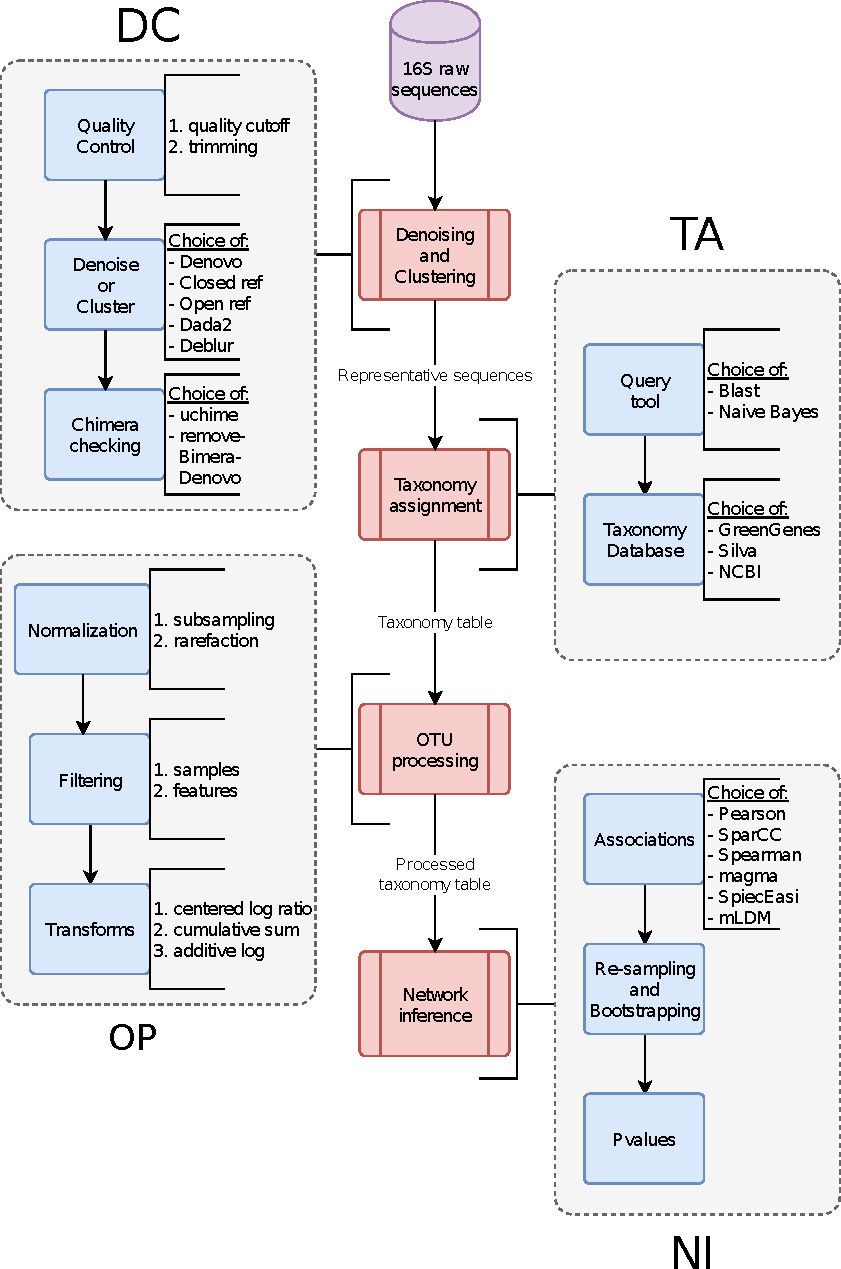
\includegraphics[width=0.69\linewidth]{figure1.pdf}
    \caption{
      \textbf{The workflow of the microbial co-occurrence analysis pipeline}.
      The steps can be grouped into four major groups: \textbf{(DC)} \textbf{D}enoising and \textbf{C}lustering, \textbf{(TA)} \textbf{T}axonomy \textbf{A}ssignment, \textbf{(OP)} \textbf{O}TU or ESV \textbf{P}rocessing, and \textbf{(NI)} \textbf{N}etwork \textbf{I}nference.
      Each step incorporates several processes, each of which in turn have several alternate algorithms for the same task (indicated by the text to the right of the blue boxes).
      The text along the arrows describes the data that is being passed from one step to another. For details on each process and data types, see Methods.
    }
    \label{fig:figure1}
  \end{figure}

  In addition to the algorithmic pipeline itself, our analysis involves two types of data: The first type consists of sets of 16S sequencing data for real communities consisting of Stool and Oral microbiomes (see Methods).
  The second are datasets artificially created for the specific goal of helping evaluate computational analysis tools.
  In particular, in order to objectively compare, to the extent possible, how well each step in \ac{micone} best captures the underlying data, we use both mock data (labelled mock4, mock12 and mock16) from mockrobiota~\cite{Bokulich2016} as well as, synthetically generated reads from an Illumina read simulator called ART~\cite{Huang2012}.
  These mock datasets consist of fake sequencing reads generated from reads obtained from synthetic microbial isolates mixed in know proportions. They contain the expected compositions along with the reference sequences for the organisms in the mock community.
  The synthetic reads were simulated using three different taxonomy distribution profiles, namely soil and water microbiomes obtained \ac{emp}~\cite{Thompson2017} and Stool microbiome that is used in our real community analysis~\cite{Kang2017}.
  Reference sequences were generated using \ac{ncbi} and the Decard package~\cite{Golob2017} for these taxonomy profiles.
  Detailed information on the mock communities and the settings used to generate the synthetic data are provided in the Methods section.


  \FloatBarrier

  \subsection*{The choice of reference database has the biggest impact on inferred networks}

  In order to analyze the effect of different statistical methods on the inferred co-occurrence networks, we generated co-occurrence networks using all possible combinations of methods and estimated the variability in the networks due to each choice.
  This analysis is performed while keeping the network inference algorithm (NI step) the same throughout the analysis.
  The effects of various steps on the final co-occurrence network is estimated by building a linear model of the edges of the network as a function the various step in the analysis pipeline (see Methods).
  Figure \ref{fig:figure2}B, shows the fraction of total variation among the co-occurrence networks due to the first three steps of the pipeline. In other words, each point corresponds to a different combination of tools, and captures how much the final network is affected by such choice.
  The 16S reference database contributes the most ($\sim25\%$) to variation in the networks. This is also reflected in the fact that the networks can be clearly separated based on the database used (Figure \ref{fig:figure2}B).
  This indicates that the taxonomy assigned to the reference sequences drastically alters the co-occurrence network and this change is much more significant than how the reference sequences themselves are identified (in the DC step).
  We believe that the grouping of the networks by taxonomy assignment into clusters (Figure~\ref{fig:figure2}B) is due to the mislabelling of constitutive taxa that are present in high abundance in the community, which drastically alters the nodes and hence the underlying network topology.
  The residual variation (Figure \ref{fig:figure2}A) can be seen as an artifact that arises when multiple steps are changed at the same time.
  Another interesting observation is that the dissimilarity between the networks decreases when the low abundance \ac{otu}s are removed from the network. This result is elaborated in detail in the denoising and clustering section.
  These results enable us to believe that the most important criterion for accurate comparative analyses of co-occurrence networks is the taxonomy reference database.

  \begin{figure}[H]
    \centering
    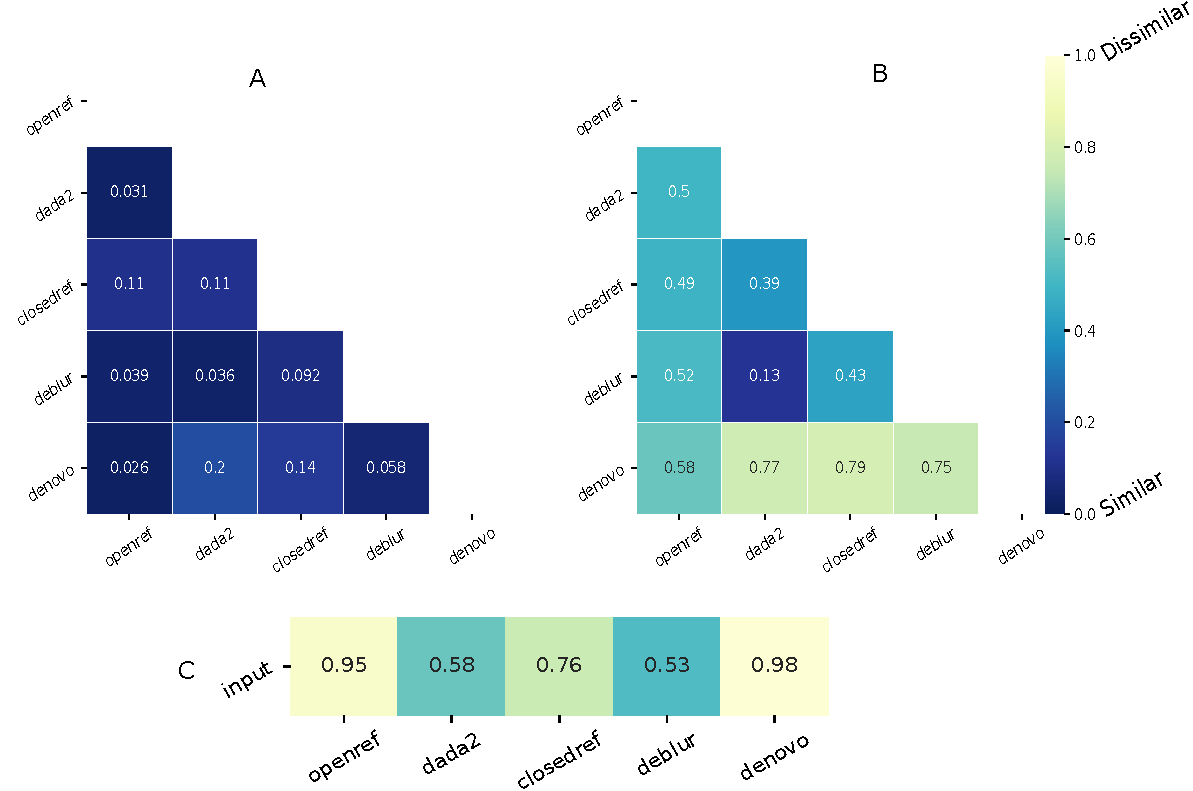
\includegraphics[width=0.85\linewidth]{figure2.pdf}
  \end{figure}
  \begin{figure}[!t]
    \centering
      \caption{
      \textbf{The choice of database contributes to the most variance in the networks}.
      \textbf{(A)} The total relative variance in the networks contributed by the DC, TA and OP steps of the pipeline (right) and the linear model used to calculate the relative variance (left), see the Methods section for details.
      \textbf{(B)} All combinations of inferred networks are shown as points on a PCA plot.
      The color of the points corresponds to the taxonomy database, the shape corresponds to the denoising/clustering method and the size corresponds to whether low abundance OTUs were removed or not.
      \textbf{(B inset)} The network generated using DC=dada2, TA=GG, OP=no and NI=SPARCC and represents the particular point shown (big red square).
      The plot clearly shows that the points can be separated based on the TA step and that the differences due to the DC and OP steps are not as significant.
    }
    \label{fig:figure2}
  \end{figure}


  \FloatBarrier

  \subsection*{Denoising and clustering methods differ in their identification of less common reference sequences}

  Denoising and clustering are commonly carried out to generate representative sequences from the raw 16S sequencing data and to obtain the \ac{otu}/\ac{esv} tables (counts of these representative sequences for each sample).
  In order to compare the \ac{otu} tables generated by different tools we processed the same 16S sequencing reads (healthy samples from a fecal microbiome transplant study~\cite{Kang2017}) using 5 different methods:  open-reference clustering, closed-reference clustering, denovo clustering, \ac{dada2}~\cite{Callahan2016} and Deblur~\cite{Amir2017}.
  The first three methods are from the \ac{qiime1}~\cite{Caporaso2010} package.
  We find that there is good agreement in the \ac{otu}/\ac{esv} tables when different combinations of methods are used to generate them (Supplementary Figure~\ref{fig:figureS1}).

  To compare the representative sequences generated by these methods we employ both the weighted~\cite{Lozupone2007} (Figure~\ref{fig:figure3}A) and unweighted UniFrac method~\cite{Lozupone2005} (Figure~\ref{fig:figure3}B).
  The weighted UniFrac distance metric takes into account the counts of the representative sequences, whereas the unweighted UniFrac distance metric does not and hence gives equal weights to each sequence.
  From Figure~\ref{fig:figure3}A one can see that the representative sequences generated by the different methods are similar to each other when weighted by their abundance.
  Figure~\ref{fig:figure3}B on the other hand shows an increase in dissimilarity between each pair of methods suggesting that the methods might differ in the treatment of sequences of low abundance.
  In order to verify this claim, for each of these methods we use the \ac{gg} taxonomy database to assign taxonomies to the representative sequences.
  We then correlate the abundances of matching taxonomies between a pair of DC methods (Figure \ref{fig:figureS1}A and B).
  The \ac{esv} tables generated by methods that perform denoising are very similar to each other $\sim0.91$ and the \ac{otu} tables generated by the clustering methods are very similar to each other $\sim0.9$, but results of denoising and clustering are highly uncorrelated with each other $\sim0.4$ (Figure \ref{fig:figureS1}C).

  These comparisons only elucidate the pairwise similarity or dissimilarity of a pair of methods.
  In order to determine the tool that most accurately recapitulates the reference sequences in the samples, we use the 16S sequences from the mock datasets.
  In particular, we used the pipeline to process mock community datasets using each of the possible methods included for this step.
  We next compared predicted representative sequences with expected representative sequences and their distribution.
  The results (Figure~\ref{fig:figure3}C and D) show that, for the mock datasets, the different methods perform similar to each other, exactly as observed in the case of the real dataset. However, the mock predicted sequence distributions are substantially different from the expected sequence distribution.
  This result is more exaggerated in the case of the unweighted UniFrac metric, where some of the datasets show a very high deviation from the expected sequences.
  These high deviations are primarily in two of the three datasets that were analyzed and show that the datasets themselves play a big role in the performance of these methods.
  This can be clearly seen in the performance (weighted UniFrac distance) of \ac{dada2} and Deblur on mock12 and mock16 datasets, where, Deblur outperforms \ac{dada2} on mock12 but the under-performs on mock16.

  There is no method that clearly outperforms the rest in all datasets.
  Based on their slightly better performance on the mock datasets, their \textit{de novo} error correcting nature and other previous studies~\cite{Nearing2018}, \ac{dada2} and Deblur seem to be in general the most reliable.
  Given the unexpected poor performance of Deblur on the synthetic data, the default algorithm in the pipeline was chosen to be \ac{dada2} (Supplementary Figure~\ref{fig:figureS3}).

  \begin{figure}
    \centering
    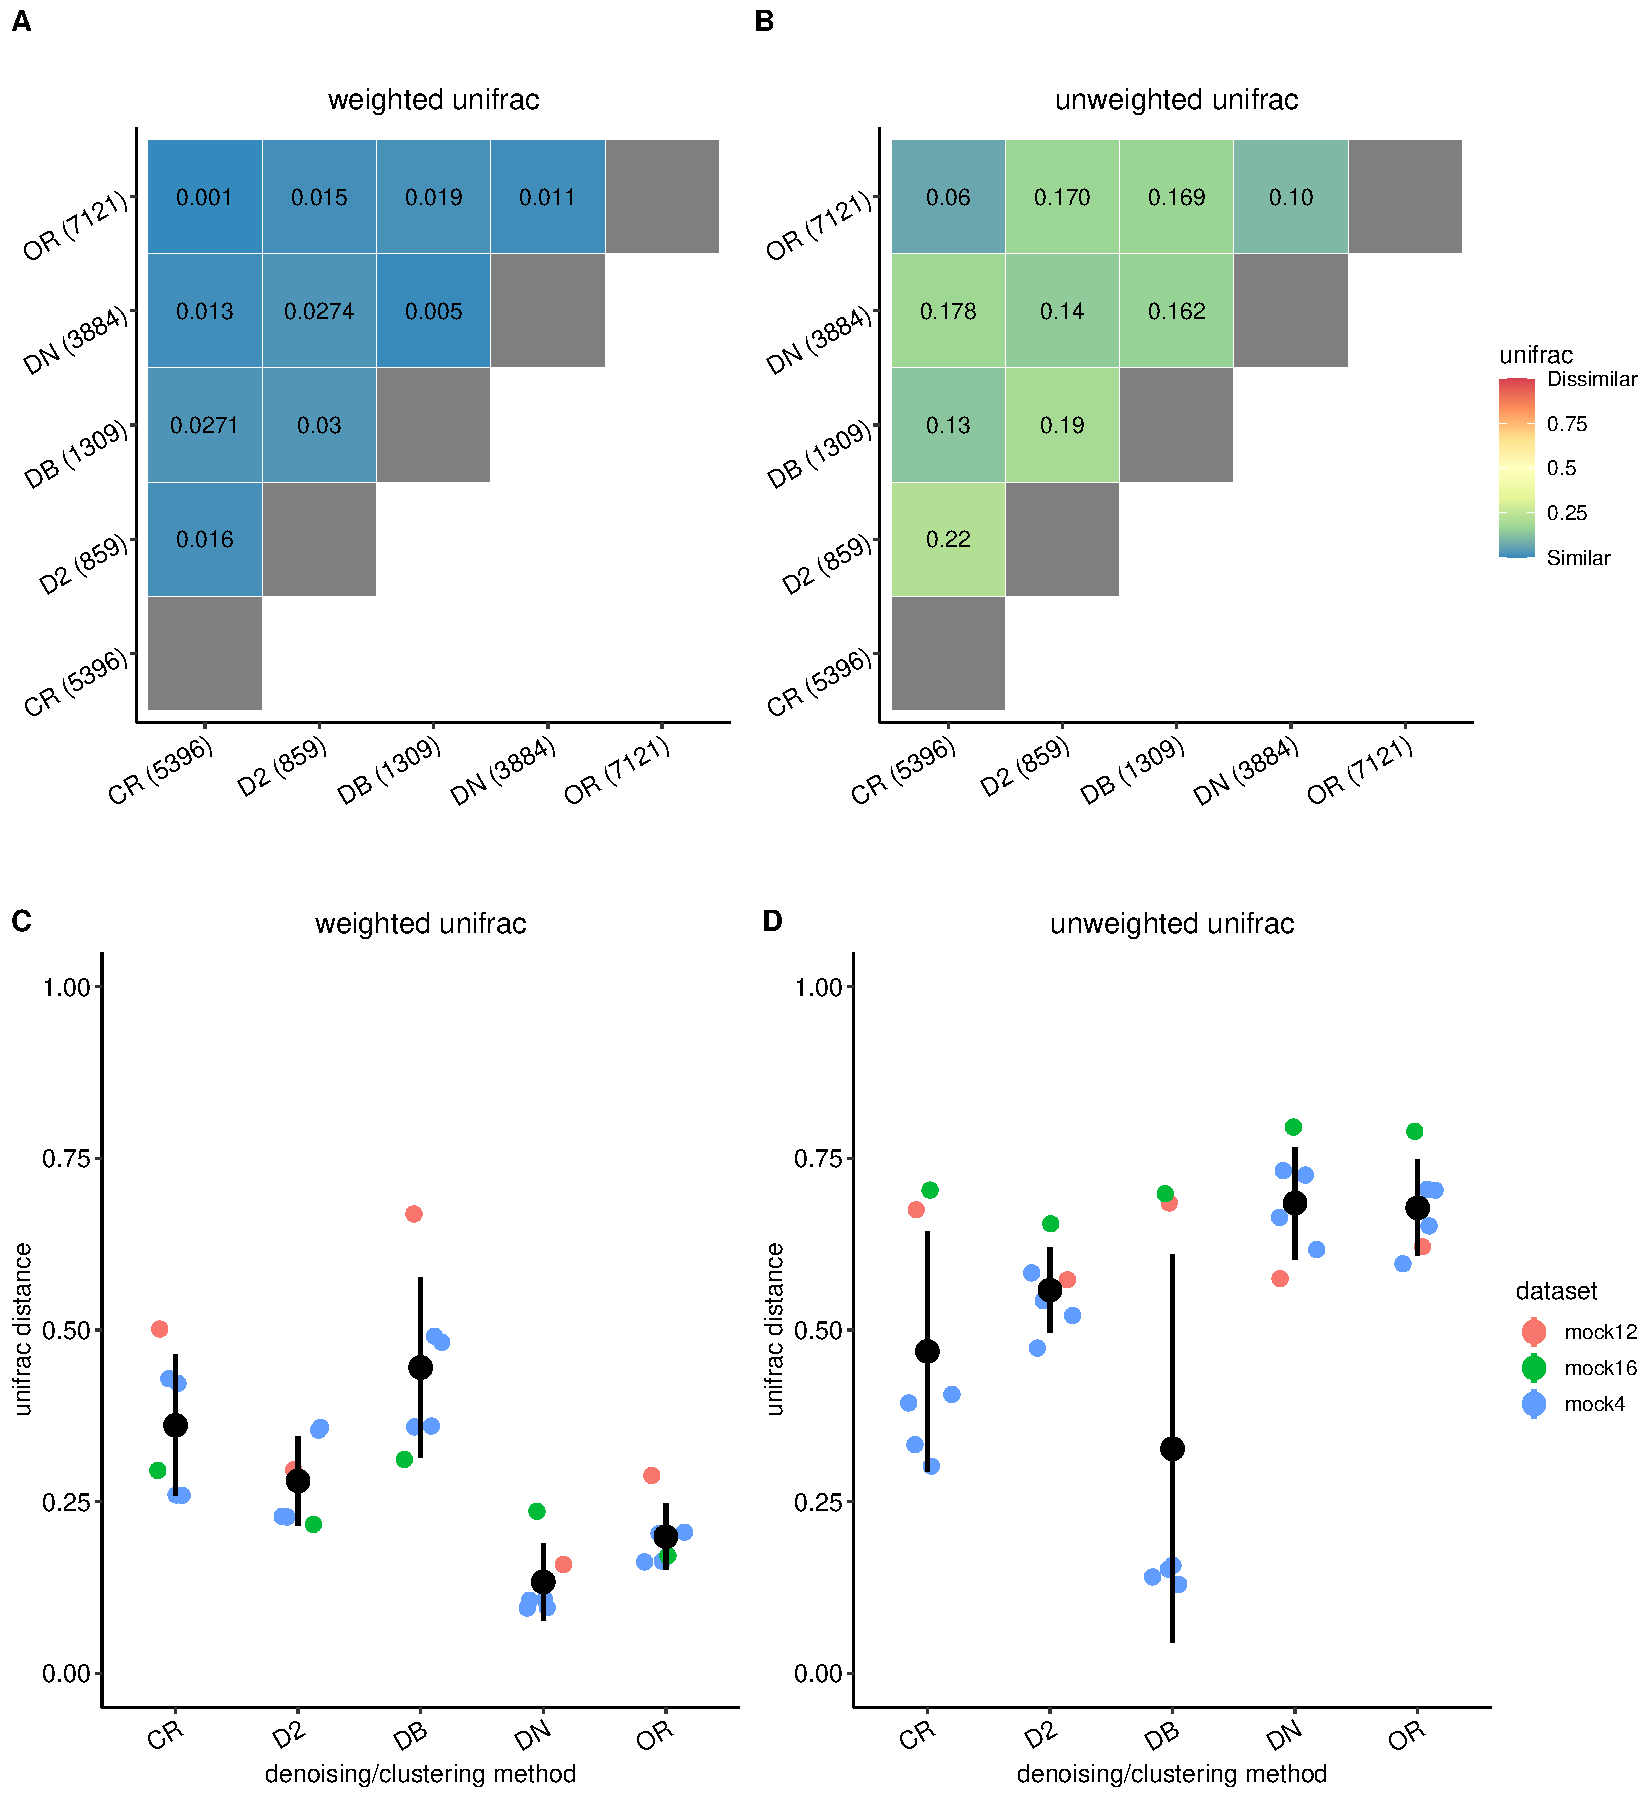
\includegraphics[width=\textwidth]{figure3.pdf}
    \caption{
      \textbf{The representative sequences generated by the different denoising/clustering methods are very similar but differ in the sequences that are in low abundance.}
      \textbf{(A)} The average weighted UniFrac distance between the representative sequences shows that the representative sequences and their compositions are fairly identical between the methods,
      \textbf{(B)} The relatively larger average unweighted UniFrac distance indicates that methods differ in their identification of sequences of low abundance,
      \textbf{(C, D)} The distributions of the avegage weighted UniFrac distance between the expected sequence profile and the calculated sequence profile in mock datasets.
      \textbf{(D)} The distributions of the average unweighted UniFrac distance show that dada2 and Deblur were the best performing methods in most of the datasets.
    }
    \label{fig:figure3}
  \end{figure}

  \FloatBarrier

  \subsection*{Taxonomy databases vary widely in taxonomy hierarchy and update frequency}

  Taxonomy databases are used to assign taxonomic identities to the representative sequences obtained after the DC step.
  In order to compare the assigned taxonomies from different databases, we use the same reference sequences and assign taxonomies to them using different taxonomy reference databases.
  The three 16S taxonomic reference databases used in this study are SILVA~\cite{Quast2012}, \ac{gg}~\cite{DeSantis2006} and \ac{ncbi} RefSeq.
  SILVA and \ac{gg} are two popular 16S databases used for taxonomy identification.
  The \ac{ncbi} RefSeq nucleotide database contains 16S rRNA sequences as a part of two BioProjects - 33175 and 33317.
  The three databases vastly differ in terms of their last update status - \ac{gg} was last updated on May 2013, SILVA was last updated on December 2017 at the time of writing and \ac{ncbi} is updated as new sequences are curated.
  Since updates to taxonomic classifications are frequent, these databases vary significantly in terms of taxonomy hierarchies including species names and phylogenetic relationships~\cite{Balvociute2017}.

  The representative sequences obtained from the \ac{dada2} method in DC step were used for taxonomic assignment using the three reference databases.
  Figure~\ref{fig:figure4}A depicts a flow diagram that shows how the top 50 representative sequences (sorted by abundance) are assigned a Genus according to the three different databases.
  We observe that not only does the assigned Genus composition vary significantly, but the percentage of unassigned representative sequences (gray) also differ.
  Even the most abundant representative sequence is assigned to an "unknown" Genus in two of the three databases.
  A representative sequence might be assigned an "unknown" Genus for one of two reasons: the first is if the taxonomy identifier associated with the sequence in the database did not contain a Genus; the second (more likely) reason is that the database contains multiple sequences that are very similar to the query (representative) sequence and the consensus algorithm (from \ac{qiime2}) is unable to assign one particular Genus at the required confidence.
  After assigning all the representative sequences to taxonomies we perform a pairwise comparison of the similarity between assignments from different databases at every taxonomic level (Figure~\ref{fig:figure4}B).
  The assignments beyond Family level (Family, Genus and Species) are very dissimilar with $<70\%$ similarity between any pair of databases.
  There are no two reference databases that are more similar than the other, with \ac{gg} and SILVA producing only marginally similar assignments compared to \ac{ncbi}.
  This implies that the taxonomy assignments from each reference database are fairly unique and is one of the reasons for a large differences in the resultant co-occurrence networks generated from different taxonomy databases.
  
  Supplementary Figure~\ref{fig:figureS4} shows that the top 20 most abundant genera in the three resulting taxonomy composition tables are different.
  For example, the most abundant genus in the \ac{gg} taxonomy table was \textit{Escherichia} whereas in the SILVA taxonomy table it was \textit{Escherichia-Shigella}.
  Although these are minor differences, when comparing a large number of taxonomy composition tables these problems are hard to diagnose.
%   The comparison of all assigned genera instead of the just the top 20 contains the same percentage of matches and mismatches, implying that there does not seem to exist a correlation between abundance and mismatch.
%   This suggests that the most abundant sequences are not necessarily the ones that are consistently matched to the same taxonomies in the different reference databases.

  As in the previous section, these comparisons only indicate similarity or dissimilarity between methods.
  In order to obtain an absolute measure of accuracy of the taxonomic assignments we use the expected reference sequences from the mock datasets as the query sequences for the databases and the expected taxonomic composition as the standard to compare against (Figure~\ref{fig:figure4}C).
  Again, we observe that none of the databases perform better than the others in absolute terms.

  Given that no database performs better than others against mock datasets, and that databases are almost equally distant from each other in terms of final output, the choice of which database to use should be driven by other reason.
  One user-specific way to choose, would be based on the known representation of taxa for the microbiome of interest (see also Discussion). Another reason could be the frequency of updates and the potential for future growth, which prompted us to set \ac{ncbi} as the \ac{micone} standard for taxonomy assignment.
 In addition to being regularly maintained and updated the \ac{ncbi} database already has the advantage that its accuracy of assignments is still comparable to the SILVA and \ac{gg} reference databases that are routinely used as reference databases.

  \begin{figure}[H]
    \centering
    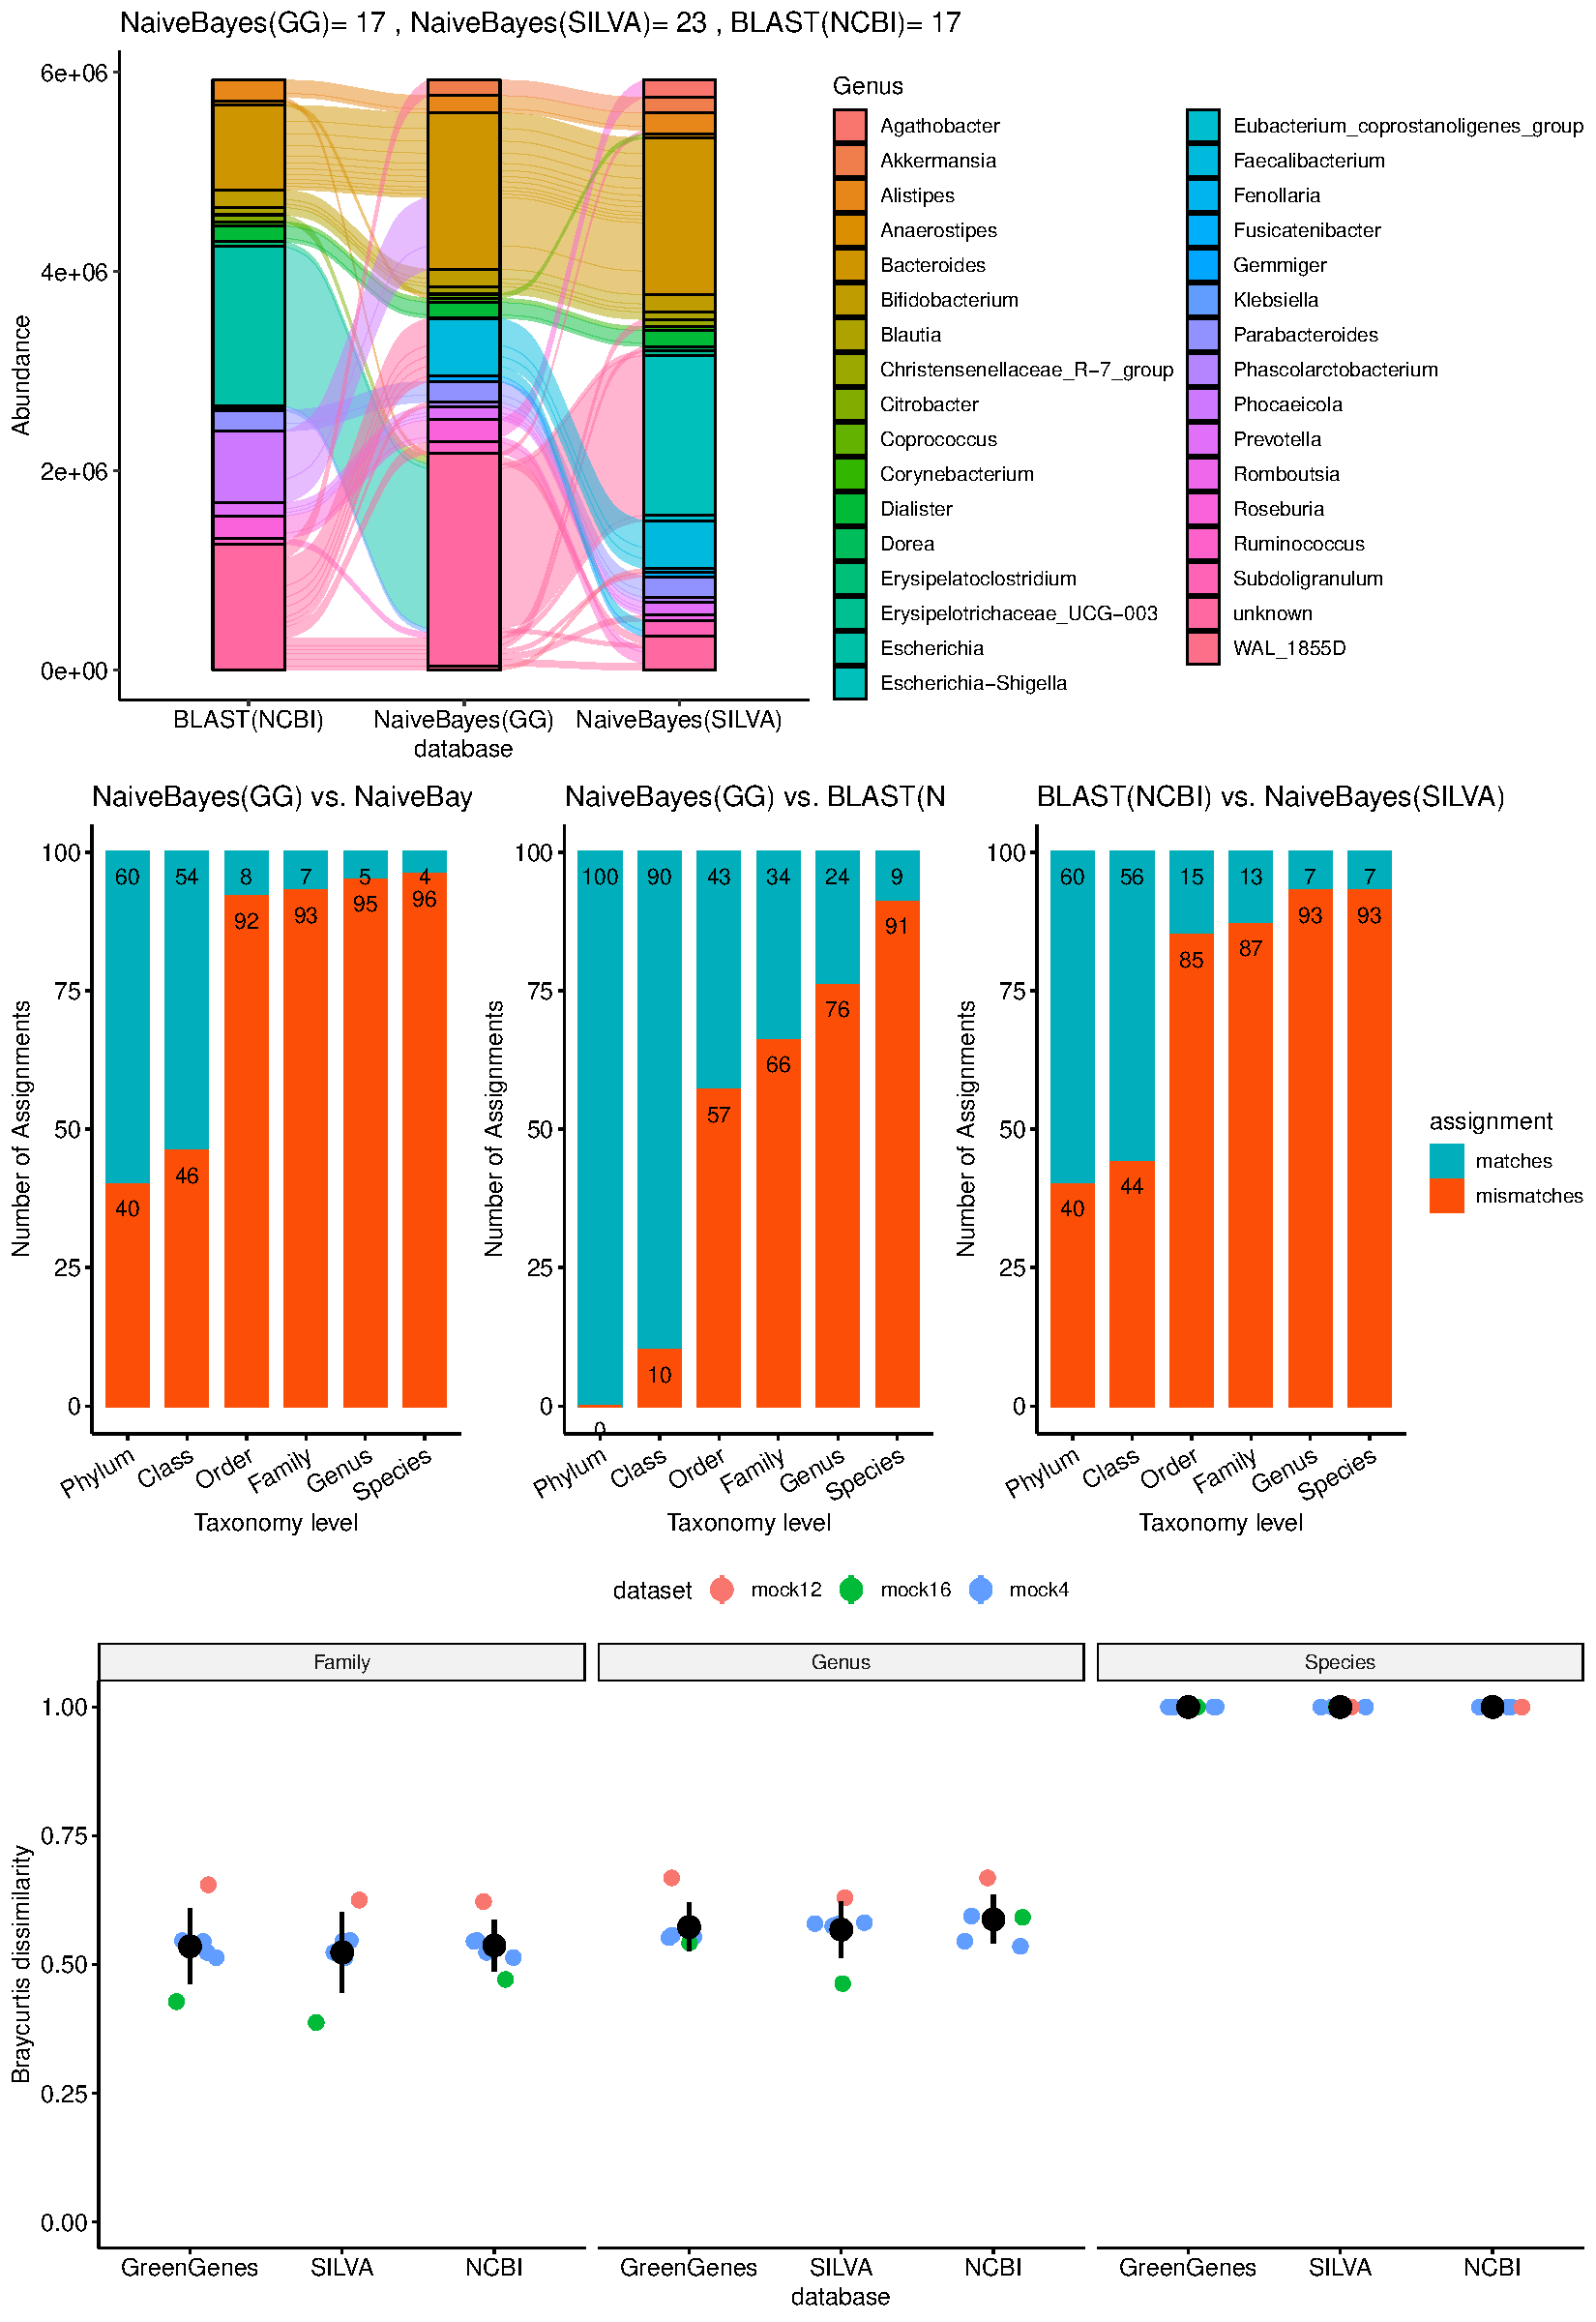
\includegraphics[width=0.9\textwidth,height=1.2\textwidth]{figure4.pdf}
  \end{figure}
  \begin{figure}[!t]
    \centering
    \caption{
      \textbf{Taxonomic reference databases vary widely in terms of their taxonomy assignments.}
      \textbf{(A)} The assignment of the top 50 representative sequences to their respective taxonomies using the three different reference databases shows how the same sequences are assigned to different Genus.
      \textbf{(B)} The percentage of \ac{otu}s assigned to the same taxonomic label when using different reference databases.
      The percentage of mismatches decrease at higher taxonomic levels but even at the Phylum level there exists around 10\% of mismatches.
      \textbf{(C)} The Bray-Curtis dissimilarity between the expected taxonomy profile and calculated taxonomy profile in the mock datasets shows that there is no singular best choice of database for every dataset.
    }
    \label{fig:figure4}
  \end{figure}

    

  \FloatBarrier

  \subsection*{Networks generated using different network inference methods show notable difference in edge-density and connectivity}

  % TODO: Talk about the difference between correlations and associations
  The six different network inference methods used in this study are \ac{magma}~\cite{Cougoul2019}, \ac{mldm}~\cite{Yang2017}, \ac{spieceasi}~\cite{Kurtz2015}, \ac{sparcc}~\cite{Friedman2012}, Spearman and Pearson.
  These network inference methods fall into two groups, the first set of methods (Pearson, Spearman, \ac{sparcc}) infer pairwise correlations while the second set infer direct associations (\ac{spieceasi}, \ac{mldm}, \ac{magma}).
  Pairwise correlation methods involve calculating the correlation coefficient between every pair of \ac{otu}/\ac{esv}s leading to the detection of spurious indirect connections.
  On the other hand, direct association methods use conditional independence to avoid the detection of correlated but indirectly connected \ac{otu}s~\cite{Kurtz2015,Menon2018}.

  For the analysis presented in this section, we used the taxonomy composition table obtained using the \ac{ncbi} reference database as the input for algorithms that infer co-occurrence associations between the microbes.
  Figure~\ref{fig:figure5}A shows the networks inferred from this dataset using the different inference algorithms.
  We can clearly see that the different networks differ vastly in their edge-density and connectivity and even some of the edges in common to these networks have their signs inverted. Note, however, that some of these comparisons depend on the threshold that has to be applied to the pairwise correlations methods (currently 0.3, based on~\cite{Friedman2012}).
  To get a more quantitative idea, we can take a look at the nodes and edges (Figure~\ref{fig:figure5}B) in common between the networks using UpSet plots~\cite{Lex} (only \ac{magma}, \ac{mldm}, \ac{spieceasi}, \ac{sparcc} are used in the comparison since Pearson and Spearman add a large number of spurious edges since they are not intended for compositional datasets).
  The results for the node intersections show that the networks have a large number of nodes in common ($63$ out of $67$ nodes in the smallest network - \ac{magma}) and no network possesses any unique node.
  The edge intersections in contrast show that only $19$ edges (out of $98$ edges in the smallest network - \ac{magma}) are in common between all the methods and each network has a large number of unique edges.
  These results indicate that there is a substantial rewiring of connections in the inferred networks.

  Unlike in the previous sections, where were we evaluated the performance of methods on mock datasets, there are no such datasets that contain a set of known interactions for the evaluation of the network inference algorithms.
  Therefore, we propose the construction of a consensus network (Figure~\ref{fig:figure5}C) involving \ac{magma}, \ac{mldm}, \ac{spieceasi} and \ac{sparcc} by merging the p-values generated from bootstraps of the original taxonomy composition table using the Browns p-value combining method~\cite{Poole} (see Methods section).
  Based on this approach, \ac{micone} reports as default output the consensus network, annotated with weights (correlations for \ac{sparcc} and direct associations for the other methods) for all four methods.

  \begin{figure}[H]
    \centering
    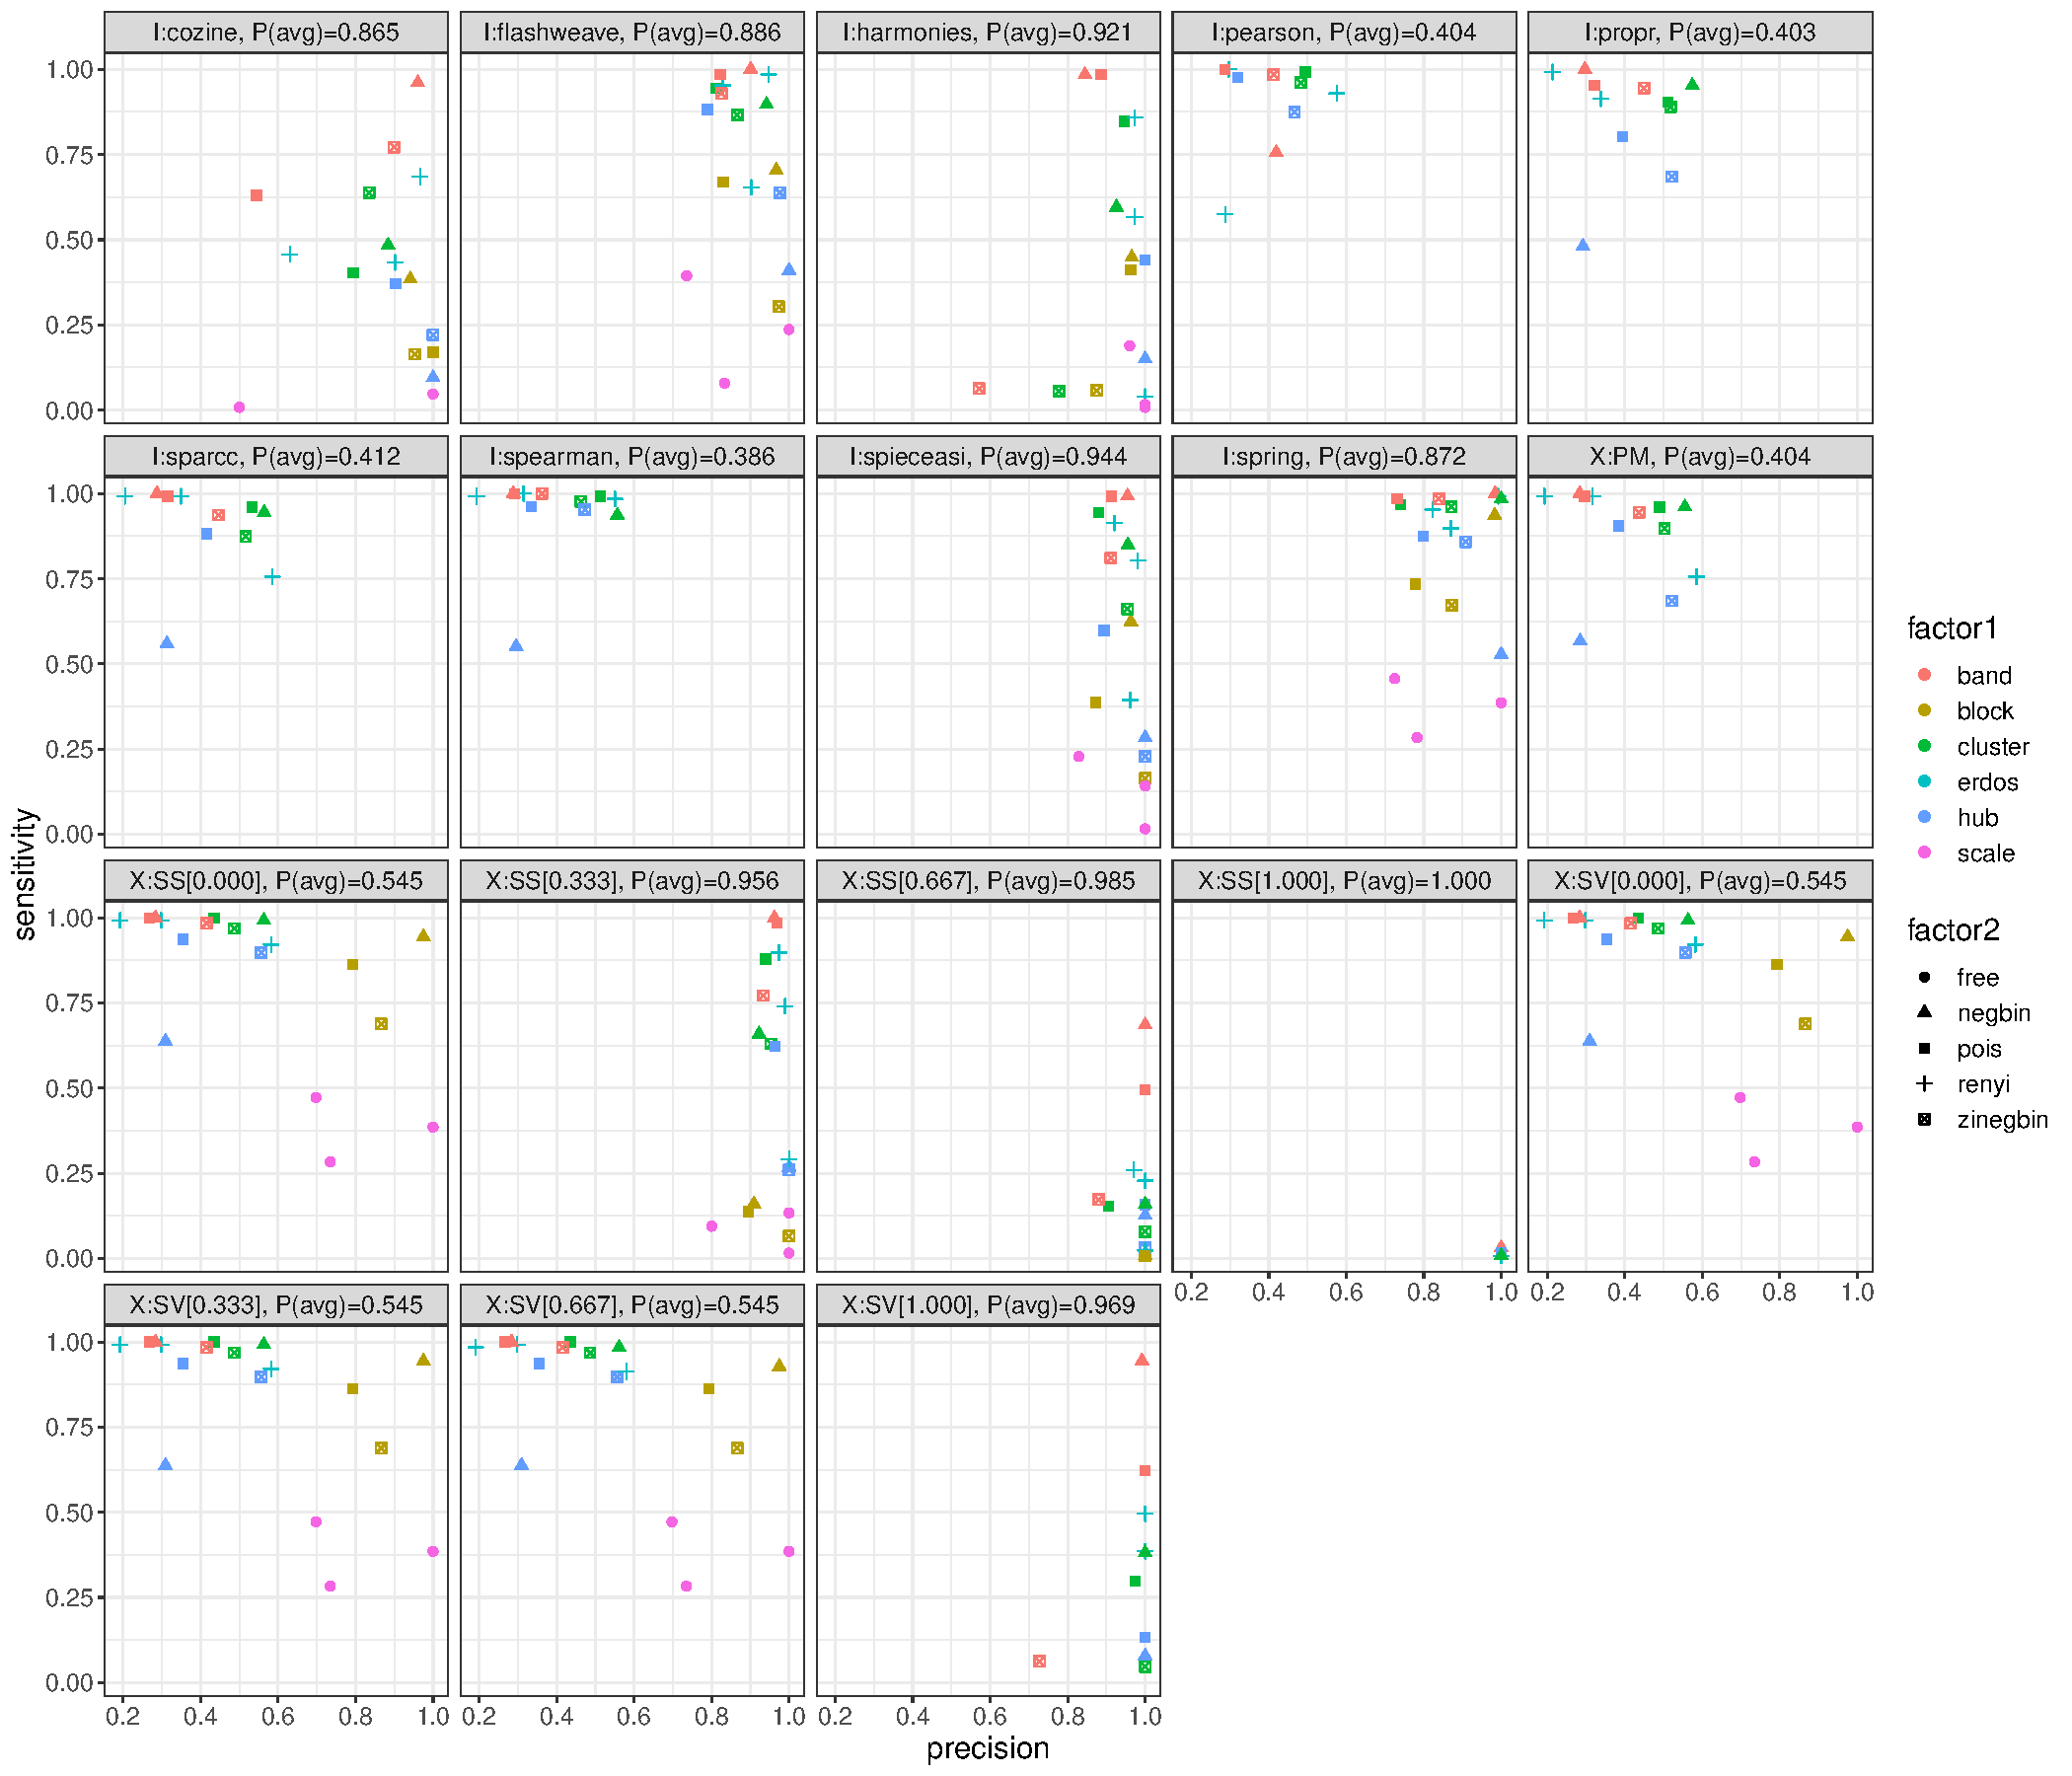
\includegraphics[width=0.9\textwidth]{figure5.pdf}
  \end{figure}
  \begin{figure}[t!]
    \centering
    \caption{
      \textbf{Networks generated using different network inference methods show notable differences both in terms of edge-density and connectivity}.
      \textbf{(A)} The six different networks generated by the different network inference methods are very dissimilar.
      The green links are positive associations and the orange links are negative associations.
      A threshold of 0.3 was set for the methods that infer pairwise correlations (\ac{sparcc}, Spearman, Pearson) and no threshold was set for the other methods.
      \textbf{(B)} The node overlap Upset plot~\cite{Lex} indicates that all the networks have a large number of common nodes involved in connections.
      Whereas, \textbf{(C)} The edge overlap Upset plot shows that a very small fraction of these connections are actually shared.
    }
    \label{fig:figure5}
  \end{figure}

 

  \FloatBarrier

  \subsubsection*{The default pipeline}
  
  The systematic analyses performed in the previous sections clearly show that the choice of tools and parameters can have a big impact on the final co-occurrence network. For some of these choices (e.g. \ac{dada2} vs. deblur) there is no clear metric to establish a best protocol.
  For other choices, the mock communities provide an opportunity to select combination of parameters that yield more accurate and robust results.
  Despite this partial degree of assessment, we wish to suggest a combination of tools and parameters that produce networks that are derived from the combination of tools which performed best on the mock communities, and displayed highest robustness to switching to alternative methods.
  These tools and parameters are chosen as the defaults for the pipeline and are given in Table~\ref{tab:default_options}.

  \begin{table}[h]
    \centering
    \small
    \begin{tabular}{|c|c|c|}
      \hline
      \textbf{Process} & \textbf{Tool} & \textbf{Parameters} \\
      \hline
      Denoising and Clustering & Dada2/Deblur & default \\
      Taxonomy Assignment & \ac{ncbi} with Blast & RefSeq database \\
      OTU Processing & Based on statistical power & Dynamic cutoff \\
      Network Inference & Consensus method & - \\
      \hline
    \end{tabular}
    \caption{Default tools and parameters for the pipeline}
    \label{tab:default_options}
  \end{table}

  The recommended tool for the \ac{dc} step (\ac{dada2} or Deblur) were chosen based on their accuracy in recapitulating the reference sequences in mock communities and synthetic data.
  The choice of the taxonomy reference database in the \ac{ta} step is dictated largely by the species expected to be present in the sample as well the database used in similar studies if comparison is a goal.
  Nevertheless, we suggest \ac{ncbi} RefSeq along with blast+ as the query tool since the database is updated regularly and has a broad collection of taxonomies.
  The abundance threshold at the \ac{op} step is determined automatically based on the number of samples and the required statistical power.
  Finally, we use the Browns p-value combining method on the networks generated using \ac{magma}, \ac{mldm}, \ac{spieceasi} and \ac{sparcc} to obtain a final consensus network in the \ac{ni} step.

  Figure~\ref{fig:figure6}A shows the default network compared against networks generated by altering one of the steps of the pipeline from the default.
  These results indicate that the biggest differences in networks occur when the reference database or the network inference algorithm are changed.
  Furthermore, the L1 distance of networks generated by altering one of the steps of the pipeline from the default against the default network (Figure~\ref{fig:figure6}B) shows that the biggest deviations from the default network occur when the \ac{ta} and \ac{ni} steps are changed, reinforcing the same results observed in Figure~\ref{fig:figure2}. Figure~\ref{fig:figure7} shows the co-occurrence networks inferred for the hard palate for healthy subjects in a periodontal disease study~\cite{Chen2018} and the healthy stool microbiome in fecal microbial transplant study~\cite{Kang2017}. These consensus networks were generated using the default tools and parameters from Table~\ref{tab:default_options}.

  \begin{figure}[h]
    \centering
    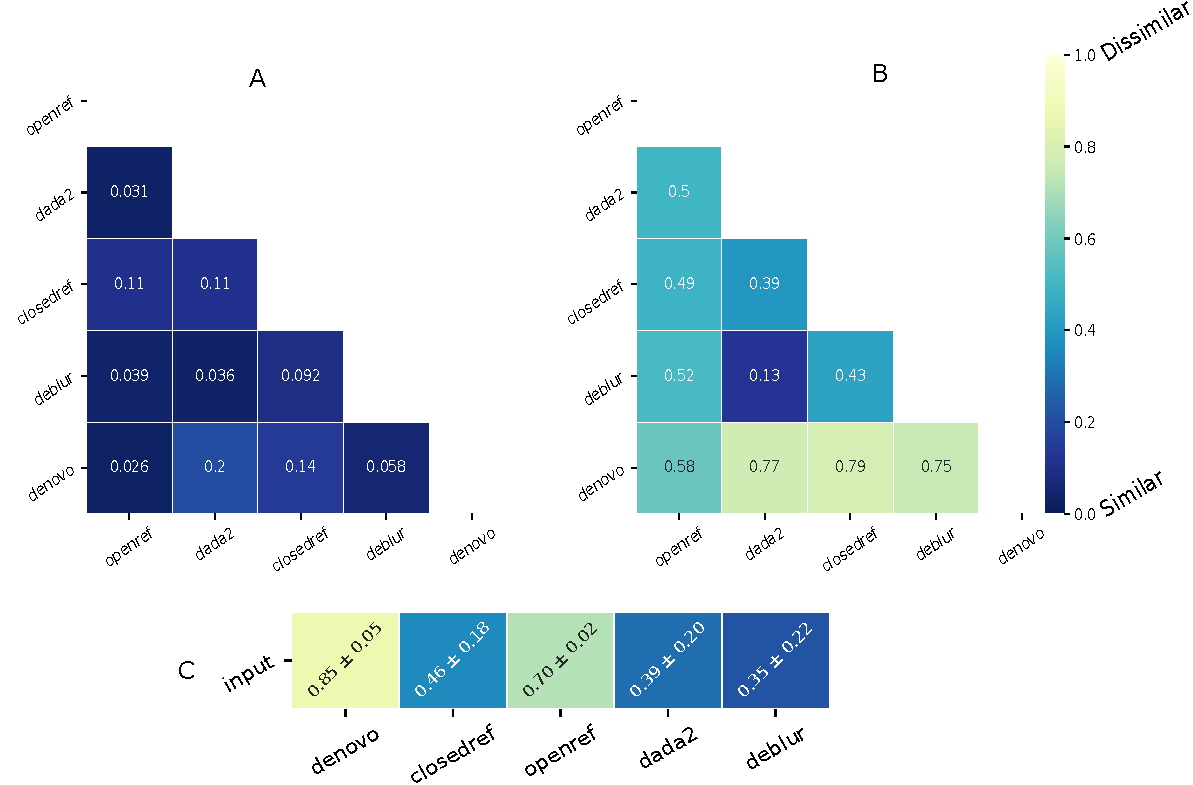
\includegraphics[width=0.85\linewidth]{figure6.pdf}
    \caption{
      \textbf{Network inference and taxonomic assignment have the highest influence on the inferred network structures.}
      \textbf{(A)} The network constructed using the default pipeline parameters (DC=\ac{dada2}, TA=\ac{ncbi}, OP=on, NI=\ac{sparcc}) is compared with networks generated when one of the steps use a different tool.
      The common connections (common with the default network) are in black, connections unique to the network are colored purple and connections in the default network but not present in the current network are gray.
      \textbf{(B)} The L1 distance between the networks generated by changing one step of the default pipeline and the network generated using the default parameters.
    }
    \label{fig:figure6}
  \end{figure}


  \begin{figure}[h]
    \centering
    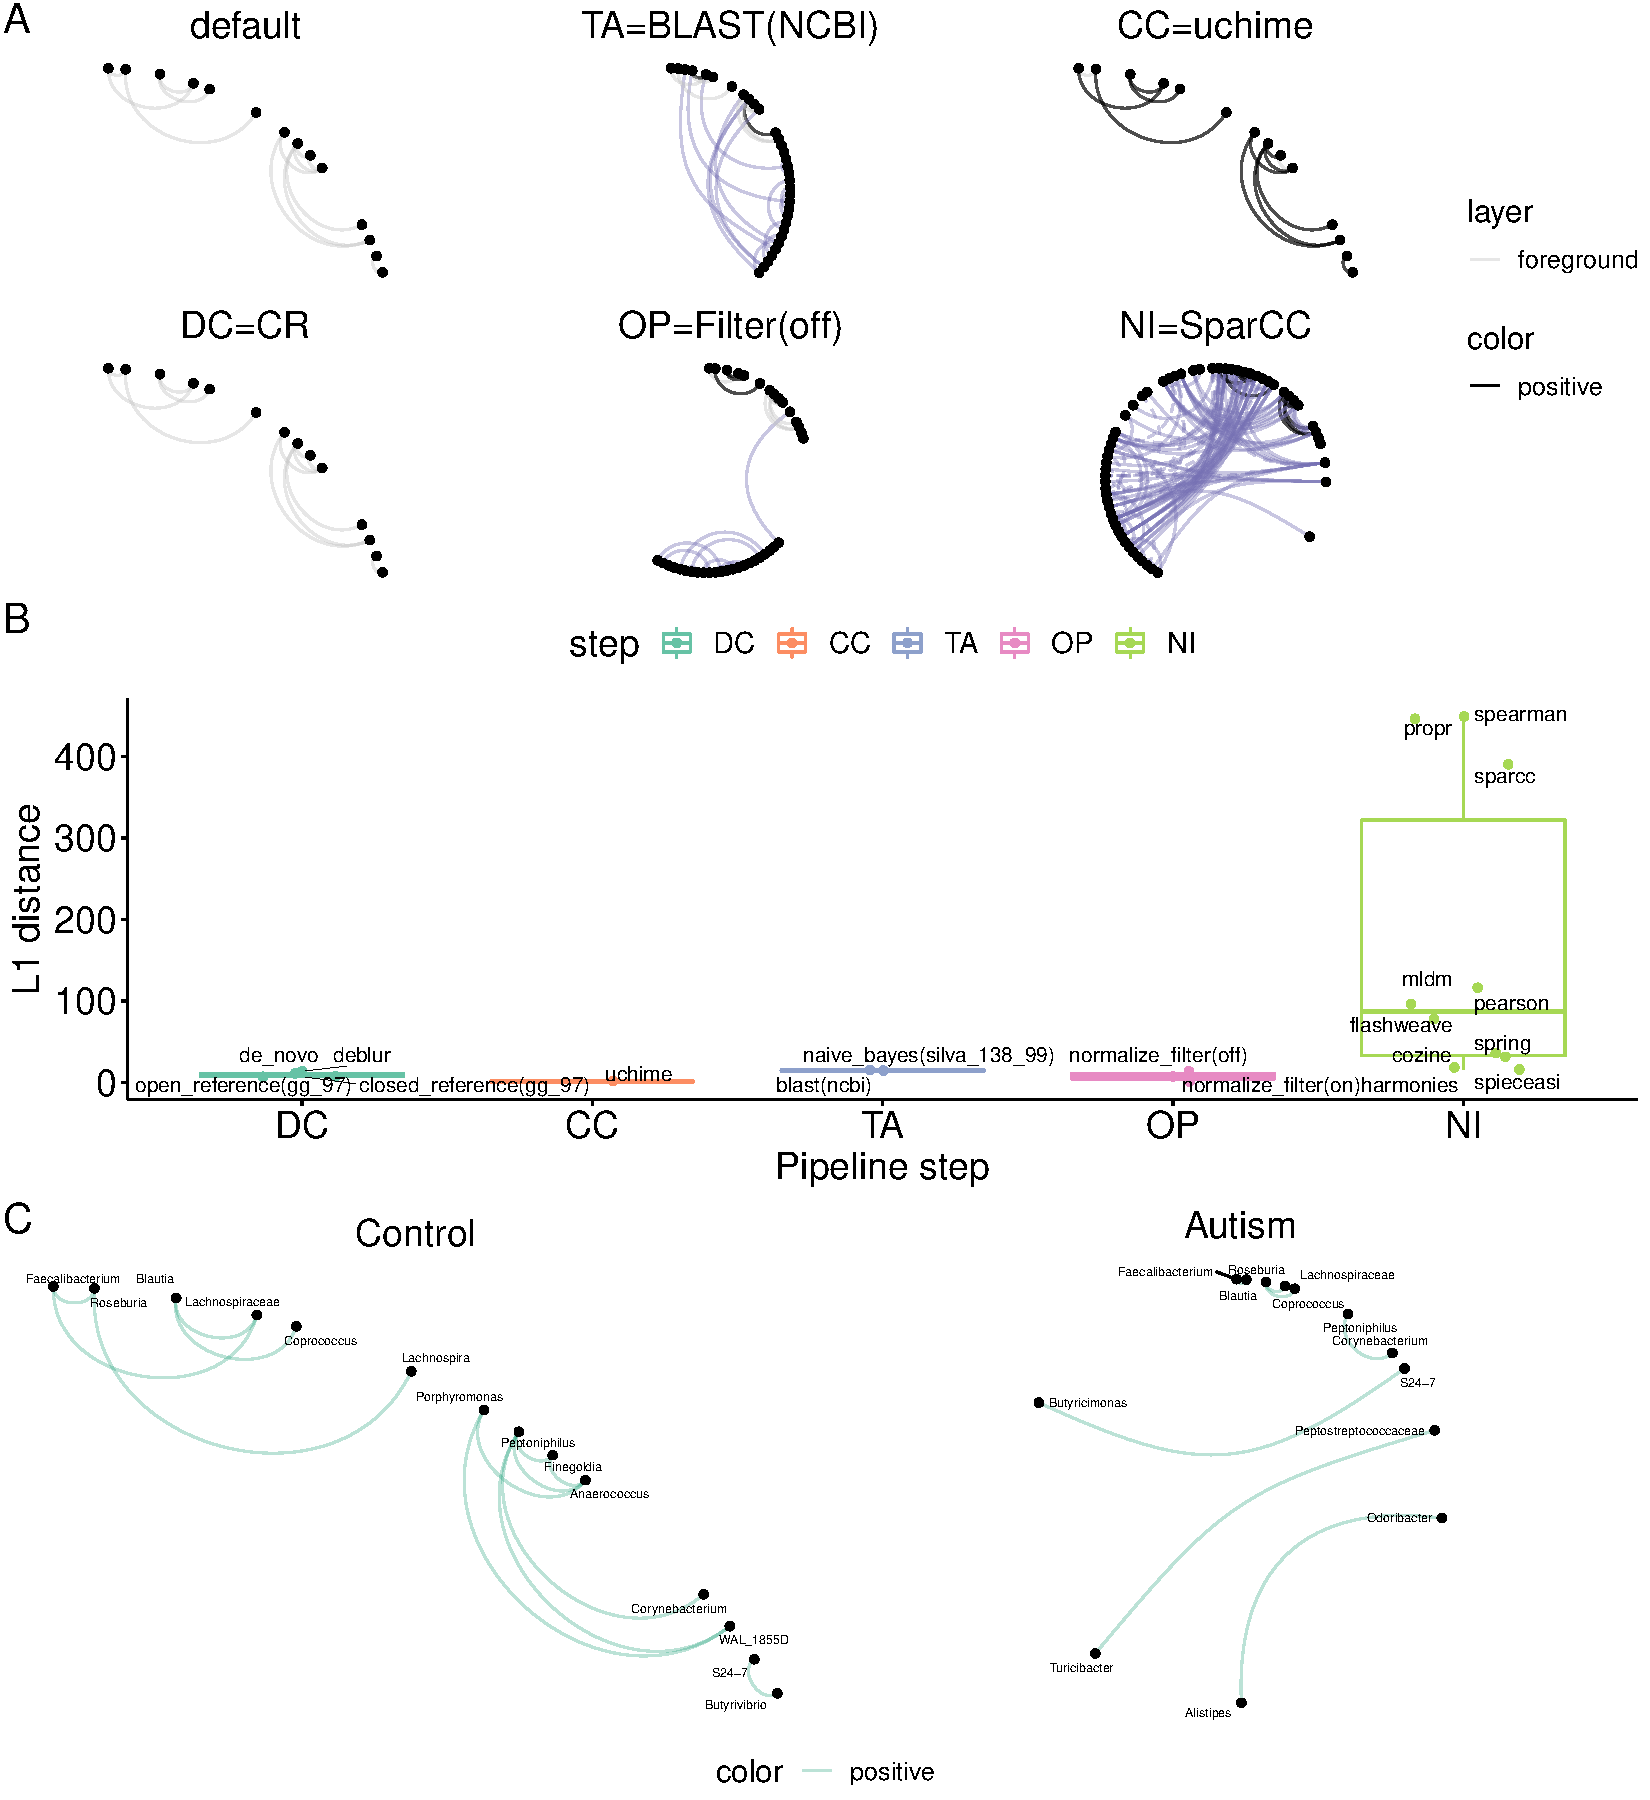
\includegraphics[width=17cm]{figure7.pdf}
    \caption{
      The consensus networks generated using the default pipeline settings.
      \textbf{(A)} Co-occurrence network of the Hard Palate microbiome generated from samples of healthy subjects in a periodontal diseases study.
      \textbf{(B)} Co-occurrence network of the Stool microbiome generated from samples of healthy subjects in a fecal microbiome transplant study.
  }
    \label{fig:figure7}
  \end{figure}


% DISCUSSION
%!TEX root = ../main.tex

\section*{Discussion}

  \subsection*{Why \ac{micone}?}

  A myriad of tools and methods have been developed for different parts of the workflow for inference of co-occurrence networks from 16S rRNA data.
  Our analyses have shown that networks generated using different combinations of tools and approaches can be substantially different from each other, highlighting the need for a clear evaluation of the source of variability and for tools that provide the most robust and accurate results.
  Our newly developed software, \ac{micone}, is a customizable pipeline for the inference of co-occurrence networks from 16S rRNA data that enables users to compare networks generated by multiple possible combinations of tools and parameters.
  Importantly, in addition to revisiting the test cases presented in this work, users will be able to explore the effect of various tool combinations on their own datasets of interest.
  The \ac{micone} pipeline has been built in a modular fashion; its plug-and-play architecture enables users to add new tools and steps, either using existing packages that have not been examined in the present work or those developed in the future.
  The \ac{micone} Python package provides functions and methods to perform a detailed analysis of the count matrices and the co-occurrence networks.
  The inferred networks are exported to a custom JSON format (see Supplementary) by default, but can also be exported to Cytoscape~\cite{shannonCytoscapeSoftwareEnvironment2003}, GML~\cite{himsoltGMLPortableGraph2010}, and many other popular formats via the Python package.

  While several tools/workflows such as \ac{qiime2}~\cite{bolyenReproducibleInteractiveScalable2019} and NetCoMi~\cite{peschelNetCoMiNetworkConstruction2020} can be used to generate co-occurrence networks from 16S sequencing data, no single tool exist that integrates the complete process of inferring microbial interaction networks from 16S sequencing reads.
  \ac{micone} is unique as it offers this functionality packaged in a workflow that can be run locally, on the compute cluster, or in the cloud.

  \subsection*{The default pipeline and recommended tools}

  Through \ac{micone}, in addition to transparently revealing the dependence of co-occurrence networks on tool and parameter choices (see Discussion in Supplementary Text for details on the DC, TA and OP steps), we have taken advantage of our spectrum of computational options and the availability of mock and synthetic datasets, to suggest a default standard setting.
  Additionally, we have developed a consensus approach, that can reliably generate networks that are fairly robust across multiple tool choices.
  An important caveat related to these results is that due to the lack of a universal standard for microbial interaction data, our conclusions are based on the specific datasets used in our analysis.
  While our analysis is based on several mock and synthetic datasets that cover a diverse range of abundance distributions and network topologies, datasets that have drastically different distributions may require a re-assessment of the best settings.

  The networks generated by different network inference methods show considerable differences in edge-density and connectivity, partially due to the underlying assumptions regarding sparsity, distribution, and compositionality.
  To address this issue, we have developed two consensus algorithms (simple voting and scaled-sum method) that generate networks whose links have evidence based on multiple inference algorithms.

 We find that the scaled-sum method performs the best on synthetic datasets, and is therefore chosen as the default for the \ac{ni} step of the pipeline.
 Notably, the consensus network displays a higher precision and returns a concise list of robust associations which represent a valuable set for experimental validation follow-up.

  \subsection*{Future directions}

  Future work building upon our current results could enhance the network inference process in multiple ways.
  The current analyses make use of one fecal microbiome transplant dataset with healthy and ASD samples, three mock community datasets, and several datasets generated by two synthetic interaction methods.
  Incorporating datasets from a broad spectrum of biomes with varying microbial distributions into \ac{micone} will likely increase the robustness and generalizability of the results from these analyses.

  The network analyses in this study are primarily at the Genus level, wherein the lowest resolution of a node is a Genus and if an entity cannot be resolved to the Genus level, the next lowest taxonomic level is used (for example, Family).
  As a consequence, two entities belonging to the same lineage where one entity is resolved to the Genus level and another is resolved to the Family level are treated as two different nodes in the network.
  Thus, the development of a metric of overlap to compare nodes with shared lineages within and across networks could enable more biologically and phylogenetically relevant comparisons.

  Although direct comparisons between co-occurrence networks and directly measured interactions are difficult to interpret and highly debated~\cite{hiranoDifficultyInferringMicrobial2019,gobernaCautionaryNotesUse2022}.
  Further, benchmarking of co-occurrence networks could also be pursued through the use of literature-based interactions~\cite{lima-mendezDeterminantsCommunityStructure2015a} or biological benchmark interaction data~\cite{sungGlobalMetabolicInteraction2017a}.
  Additionally, \ac{micone} could be extended to enable the processing of metagenomics sequencing data, facilitating the analysis of a much larger and diverse range of datasets and domains of life.

  Although in the current analysis, we have only used default parameter values recommended by the tool creators, the \ac{micone} pipeline could be used in the future to explore any combinations of parameters and to optimize these values for improved network inference.
  Overall, there likely is no ``best method'' for the various steps of 16S data analysis, and hence, \ac{micone} is intended to help researchers to identify the methods and algorithms that are most suitable for their datasets in an easy-to-use and reproducible manner.

  We envision that \ac{micone}, and its underlying tools and databases, will be increasingly useful for building large comparative analyses across studies.
  It enables rapid, configurable, and reproducible inference of microbial networks and furthers the formulation of hypotheses about the role of these interactions on community composition and stability.
  These comparative analyses will require coupled network analysis and visualization tools (such as \ac{mind}~\cite{huResourceComparisonIntegration2022}) and need systematic access to datasets, shared in accordance with FAIR standards~\cite{pachecoFAIRRepresentationsMicrobial2022}.


% METHODS
%!TEX root = ../main.tex

\section*{Materials and Methods}

  \subsection*{Datasets}

    \vspace{-5mm}
    \begin{itemize}
      \item The mock community 16S datasets were obtained from mockrobiota \cite{Bokulich2016}. We used samples (\hl{enter id number}) for this study.
      \item The real datasets were control samples (49samples) \todo[size=\footnotesize]{Check the exact number} of a fecal microbiome transplant study obtained from \cite{Kang2017}.
      \item Simulated data was generated using Grinder \cite{Angly2012}.
    \end{itemize}


  \subsection*{16S processing pipeline}

    \vspace{-5mm}

    The flowchart describing the workflow of the 16S data-analysis pipeline is as shown in Figure \ref{fig:mind_pipeline}.
    The pipeline (\hl{github link here}) integrates many publicly available tools as well as custom Python modules and scripts to extract co-occurrence associations from 16S sequence data.
    The input to the pipeline by default is the raw community 16S rRNA sequence data, but it can additionally be configured to use processed sequences, \ac{otu} tables or other types of intermediate data.
    The final output of the pipeline is the inferred network of co-occurrence relationships among the microbes present in the samples.

    Some key features of the pipeline include modularity, flexibility and ease-of-use.
    The entire pipeline consists of modules which can be modified, reordered or replaced appropriately using a simple configuration script.
    The configuration script lists the steps to be performed during runtime, along with the parameters to be used (optional) for the various steps.
    Since the entire pipeline run-through is stored in the form of a text file (the configuration file), subsequent runs are highly reproducible and changes can be easily tracked using version control.
    The pipeline allows for automatic parallelization of all possible processes, both within and across samples.
    In addition to the Python package, the entire pipeline has been containerized into a Docker \cite{Merkel1994} image (\hl{dockerhub link}) for easy deployment and setup.
    The main components of the pipeline are detailed in the following sections.

    \todo[size=\footnotesize]{Should be in the supplementary section}
    \subsubsection*{Denoising and Clustering}
      \vspace{-5mm}
      This module deals with processing the raw 16S sequence data into \ac{otu} or \ac{esv} count tables.
      It consists of three processes:
      \begin{itemize}
        \item The quality control process handles the demultiplexing and quality control steps such as trimming adapters and trimming low-quality nucleotide stretches from the sequences.
        \item The denoise/cluster process handles the conversion of the demultiplexed, trimmed sequences into \ac{otu} or \ac{esv} count tables (some methods perform clustering and taxonomy assignment in the same step).
        \item The chimera checking process handles the removal of chimeric sequences created during the \ac{pcr} step.
      \end{itemize}
      The output of this module is a counts matrix that describes the number of reads of a particular \ac{otu} or \ac{esv} (rows of the matrix) present in each sample (columns of the matrix). The pipeline incorporates \ac{qiime1} \cite{Caporaso2010}, \ac{qiime2}, \ac{dada2} \cite{Callahan2016} and Deblur \cite{Amir2017} tools in this module.

    \subsubsection*{Taxonomy Assignment}
      \vspace{-5mm}
      This module deals with assigning taxonomies to either the representative sequences of the \ac{otu}s or directly to the \ac{esv}s.
      In order to assign taxonomies to a particular sequence we use:
      \begin{itemize}
        \item A taxonomy database, which is a collection of 16S sequences of known organisms.
        \item A query tool, which allows one to compare a sequence of interest to all the sequences in the database to find the best match.
      \end{itemize}
      The pipeline incorporates \ac{gg} \cite{DeSantis2006}, SILVA \cite{Quast2012} and the \ac{ncbi} \cite{Sayers2009} databases for taxonomy assignment

    % TODO: Add Gabriel's new stuff here
    \subsubsection*{OTU and ESV Processing}
      \vspace{-5mm}
      This module deals with normalization, filtering and applying transformations on the \ac{otu} or \ac{esv} counts matrix.
      \begin{itemize}
        \item Rarefaction is a normalization technique used to overcome the bias that might arise due to variable sampling depth in different samples. This is performed either by sub-sampling or by normalization of the matrix to the lowest sampling depth.
        \item Filtering is performed to remove samples or features (\ac{otu}s or \ac{esv}s) from the count matrix that are sparse. In order to determine the filtering threshold we fix the number of samples and correlation detection power needed  and determine the number of features to be used.
        \item Transformations are performed in order to correct for and overcome the compositional bias that is inherent in a counts matrix (in most cases this is handled by the network inference algorithm).
      \end{itemize}

    \subsubsection*{Network Inference}
      \vspace{-5mm}
      This module deals with the inference of co-occurrence associations from the \ac{otu} or \ac{otu} counts matrix. These associations can be represented as a network, with nodes representing taxonomies and edges the association between them.
      \begin{itemize}
        \item A null model is created by re-sampling and bootstrapping the correlation/interaction matrix
        \item Significance of these associations is determined by calculating pvalues against this null model.
      \end{itemize}
      The pipeline includes Pearson, Spearman and \ac{sparcc} \cite{Friedman2012} as the pairwise correlation metrics, and \ac{spieceasi} \cite{Kurtz2015}, \ac{mldm} \cite{Yang2017} and \ac{daa} \cite{Menon2018} as the direct interaction metrics.

  \subsection*{Statistical Analysis of Count Matrices}

   \textbf{Taxonomy comparisons}

    \textbf{Power calculations}

  \subsection*{Statistical Analysis of Co-occurrence Networks}

    \textbf{Network Variability}:
    In order to determine the best combination of tools for the pipeline, we examine the effects of each tool on the final co-occurrence network.
    We can then estimate the variance contributed by each step in the pipeline to the total variance present across the networks.
    \begin{itemize}
      \item The distance metric used
      \item How we determine the mean network
      \item ANOVA?
    \end{itemize}

    \textbf{P-value merging}
    We then use a p-value merging strategy (refer to the CoNet paper)

  \subsection*{MIND Data Visualizer}

    The data visualizer facilitates easy visualization and exploration of the data generated by the pipeline.
    This tool is a Python web-based interface built using dash \cite{dash}.
    It aids in the analysis of the effects of different processing methods on the generated counts matrix or network.
    The data from a pipeline run can be directly fed into the visualizer, allowing one to visualize various properties of intermediate \ac{otu} or \ac{esv} tables and final association networks.
    This tool makes it easy and straightforward to compare different methods and combinations of methods in the 16S data analysis workflow. The visualization tool supports:
    \begin{itemize}
      \item Filtering and aggregating data from multiple sources (data-sets)
      \item Comparing properties of the generated counts matrices and networks across different methods
      \item Visualization of these properties
    \end{itemize}

  \subsection*{Code and Data Availability}

    Links here


% ACKNOWLEDGMENTS
%!TEX root = ../main.tex

% TODO: Update this section
\section*{Acknowledgments}

We are grateful to members of the Segrè lab for helpful discussions and for feedback on the manuscript. This work was partially funded by grants from the Defense Advanced Research Projects Agency (Purchase Request No. HR0011515303, Contract No. HR0011\-15\-C\-0091), the U.S. Department of Energy (DE\-SC0012627), the NIH (T32GM100842, 5R01DE024468, R01GM121950 and Sub\_P30DK036836\_P\&F), the National Science Foundation (1457695), the Human Frontiers Science Program (RGP0020/2016), and the Boston University Interdisciplinary Biomedical Research Office. [DANIEL, KIRILL: MISSING GRANTS???] 

\section*{Contributions}


%--------------------------------------------------------%
%   REFERENCE LIST
%--------------------------------------------------------%
\newpage
\singlespacing
\printbibliography

%--------------------------------------------------------%
%   APPENDIX
%--------------------------------------------------------%

%!TEX root = ../main.tex

\begin{acronym}[XXXXXXXX]
    \acro{ngs}[NGS]{next-generation sequencing}
    \acro{mind}[MIND]{Microbial Interaction Network Database}
    \acro{micone}[MiCoNE]{Microbial Co-occurrence Network Explorer}
    \acro{otu}[OTU]{Operational Taxanomic Unit}
    \acro{esv}[ESV]{Exact Sequence Variant}
    \acro{pcr}[PCR]{Polymerase Chain Reaction}
    \acro{emp}[EMP]{Earth Microbiome Project}
    \acro{gg}[GG]{Greengenes}
    \acro{ncbi}[NCBI]{National Center for Biotechnology Information}
    \acro{comets}[COMETS]{Computation of Microbial Ecosystems in Time and Space}
    \acro{dada2}[DADA2]{Divisive Amplicon Denoising Algorithm 2}
    \acro{qiime1}[QIIME1]{Quantitative Insights Into Microbial Ecology 1}
    \acro{qiime2}[QIIME2]{Quantitative Insights Into Microbial Ecology 2}
    \acro{sparcc}[SparCC]{Sparse Correlations for Compositional data}
    \acro{spieceasi}[SpiecEasi]{Sparse InversE Covariance estimation for Ecological Association and Statistical Inference}
    \acro{mldm}[mLDM]{metagenomic Lognormal-Dirichlet-Multinomial}
    \acro{cozine}[COZINE]{COmpositional Zero-Inflated Network Estimation}
    \acro{spring}[SPRING]{Semi-Parametric Rank-based approach for INference in Graphical model}
    \acro{harmonies}[HARMONIES]{Hybrid Approach for Microbiome Networks Inference via Exploiting Sparsity}
    \acro{kegg}[KEGG]{Kyoto Encyclopedia of Genes and Genomes}
    \acro{fba}[FBA]{Flux Balance Analysis}
    \acro{sp}[SP]{Sequence Processing}
    \acro{dc}[DC]{Denoising and Clustering}
    \acro{ta}[TA]{Taxonomy Assignment}
    \acro{op}[OP]{OTU Processing}
    \acro{ni}[NI]{Network Inference}
\end{acronym}

%!TEX root = ../main.tex

\newpage
\section*{Supplementary}

  \renewcommand{\thefigure}{S\arabic{figure}}
  \setcounter{figure}{0}

  \renewcommand{\thetable}{S\arabic{table}}
  \setcounter{table}{0}

  \begin{table}[H]
\centering
\small
\begin{tabular}{|c|c|c|c|c|}
\hline
\textbf{Step}                         & \textbf{Task}                   & \textbf{Module}                                   & \textbf{Parameter}           & \textbf{Value}   \\ \hline
\multirow{14}{*}{Sequence Processing} & \multirow{6}{*}{Demultiplexing} & \multirow{3}{*}{demultiplexing\_illumina\_single} & barcode\_column              & barcode-sequence \\
                                      &                                 &                                                   & rev\_comp\_barcodes          & false            \\
                                      &                                 &                                                   & rev\_comp\_mapping\_barcodes & false            \\ \cline{3-5}
                                      &                                 & \multirow{3}{*}{demultiplexing\_illumina\_paired} & barcode\_column              & barcode-sequence \\
                                      &                                 &                                                   & rev\_comp\_barcodes          & false            \\
                                      &                                 &                                                   & rev\_comp\_mapping\_barcodes & false            \\ \cline{2-5}
                                      & \multirow{8}{*}{Trimming}       & export\_visualization\_single                     & seq\_samplesize              & 10000            \\ \cline{3-5}
                                      &                                 & export\_visualization\_paired                     & seq\_samplesize              & 10000            \\ \cline{3-5}
                                      &                                 & \multirow{3}{*}{trimming\_single}                 & ncpus                        & 1                \\
                                      &                                 &                                                   & max\_ee                      & 2                \\
                                      &                                 &                                                   & trunc\_q                     & 2                \\ \cline{3-5}
                                      &                                 & \multirow{3}{*}{trimming\_paired}                 & ncpus                        & 1                \\
                                      &                                 &                                                   & max\_ee                      & 2                \\
                                      &                                 &                                                   & trunc\_q                     & 2                \\ \hline
\end{tabular}
\caption{The default parameters used in the Sequence Processing step of the \ac{micone} pipeline}
\label{tab:sp_parameters}
\end{table}

\begin{table}[H]
\centering
\small
\begin{tabular}{lllll}
\hline
\textbf{Step}                             & \textbf{Task}                                            & \textbf{Tool}                          & \textbf{Parameter}                     & \textbf{Value}                                                                                           \\ \hline
\multirow{17}{*}{Sequence Processing}     & \multirow{4}{*}{Bootstrap}                               & \multirow{3}{*}{resample}              & bootstraps                             & 1000                                                                                                     \\
                                          &                                                          &                                        & ncpus                                  & 1                                                                                                        \\
                                          &                                                          &                                        & filter\_flag                           & True                                                                                                     \\
                                          &                                                          & pvalue                                 & ncpus                                  & 1                                                                                                        \\ \cline{2-5}
                                          & \multirow{12}{*}{Correlation}                            & \multirow{2}{*}{sparcc}                & iterations                             & 50                                                                                                       \\
                                          &                                                          &                                        & ncpus                                  & 1                                                                                                        \\
                                          &                                                          & pearson                                & -                                      & -                                                                                                        \\
                                          &                                                          & spearman                               & -                                      & -                                                                                                        \\
                                          &                                                          & \multirow{5}{*}{spieceasi}             & method                                 & mb                                                                                                       \\
                                          &                                                          &                                        & ncpus                                  & 1                                                                                                        \\
                                          &                                                          &                                        & nreps                                  & 50                                                                                                       \\
                                          &                                                          &                                        & nlambda                                & 20                                                                                                       \\
                                          &                                                          &                                        & lambda\_min\_ratio                     & 1e-2                                                                                                     \\
                                          &                                                          & \multirow{2}{*}{mldm}                  & z\_mean                                & 1                                                                                                        \\
                                          &                                                          &                                        & max\_iteration                         & 1500                                                                                                     \\
                                          &                                                          & magma                                  & -                                      & -                                                                                                        \\ \cline{2-5}
                                          & Network                                                  & make\_network                          & -                                      & -                                                                                                        \\ \hline
\end{tabular}
\caption{The default parameters used in the various tools of the pipeline}
\label{tab:all_parameters}
\end{table}

\begin{table}[H]
\centering
\small
\begin{tabular}{lllll}
\hline
\textbf{Step}                             & \textbf{Task}                                            & \textbf{Tool}                          & \textbf{Parameter}                     & \textbf{Value}                                                                                           \\ \hline
\multirow{29}{*}{Denosing and Clustering} & \multicolumn{1}{c}{\multirow{9}{*}{Sequence Processing}} & \multirow{2}{*}{join\_reads}           & min\_overlap                           & 6                                                                                                        \\
                                          & \multicolumn{1}{c}{}                                     &                                        & perc\_max\_diff                        & 8                                                                                                        \\
                                          & \multicolumn{1}{c}{}                                     & \multirow{2}{*}{demultiplex\_illumina} & rev\_comp\_barcodes                    & False                                                                                                    \\
                                          & \multicolumn{1}{c}{}                                     &                                        & rev\_comp\_mapping\_barcodes           & False                                                                                                    \\
                                          & \multicolumn{1}{c}{}                                     & demultiplex\_454                       & -                                      & -                                                                                                        \\
                                          & \multicolumn{1}{c}{}                                     & \multirow{4}{*}{trim\_filter\_fixed}   & seq\_sample\_size                      & 10,000                                                                                                   \\
                                          & \multicolumn{1}{c}{}                                     &                                        & ncpus                                  & 1                                                                                                        \\
                                          & \multicolumn{1}{c}{}                                     &                                        & trunc\_q                               & 2                                                                                                        \\
                                          & \multicolumn{1}{c}{}                                     &                                        & max\_ee                                & 2                                                                                                        \\ \cline{2-5}
                                          & \multirow{3}{*}{Chimera Checking}                        & uchime                                 & -                                      & -                                                                                                        \\
                                          &                                                          & \multirow{2}{*}{remove\_bimera}        & ncpus                                  & 1                                                                                                        \\
                                          &                                                          &                                        & chimera\_method                        & consensus                                                                                                \\ \cline{2-5}
                                          & \multirow{17}{*}{Denoise Cluster}                        & \multirow{3}{*}{de\_novo}              & enable\_rev\_strand\_match             & True                                                                                                     \\
                                          &                                                          &                                        & suppress\_de\_novo\_chimera\_detection & True                                                                                                     \\
                                          &                                                          &                                        & ncpus                                  & 1                                                                                                        \\
                                          &                                                          & \multirow{4}{*}{closed\_reference}     & enable\_rev\_strand\_match             & True                                                                                                     \\
                                          &                                                          &                                        & suppress\_de\_novo\_chimera\_detection & True                                                                                                     \\
                                          &                                                          &                                        & ncpus                                  & 1                                                                                                        \\
                                          &                                                          &                                        & reference\_sequences                   & 97\_otus.fasta                                                                                           \\
                                          &                                                          & \multirow{5}{*}{open\_reference}       & enable\_rev\_strand\_match             & True                                                                                                     \\
                                          &                                                          &                                        & suppress\_de\_novo\_chimera\_detection & True                                                                                                     \\
                                          &                                                          &                                        & ncpus                                  & 1                                                                                                        \\
                                          &                                                          &                                        & reference\_sequences                   & 97\_otus.fasta                                                                                           \\
                                          &                                                          &                                        & picking\_method                        & uclust                                                                                                   \\
                                          &                                                          & \multirow{2}{*}{dada2}                 & ncpus                                  & 1                                                                                                        \\
                                          &                                                          &                                        & big\_data                              & FALSE                                                                                                    \\
                                          &                                                          & \multirow{3}{*}{deblur}                & ncpus                                  & 1                                                                                                        \\
                                          &                                                          &                                        & mind\_reads                            & 2                                                                                                        \\
                                          &                                                          &                                        & min\_size                              & 2                                                                                                        \\ \hline
\end{tabular}
\caption{The default parameters used in the various tools of the pipeline}
\label{tab:all_parameters}
\end{table}


\begin{table}[H]
\centering
\small
\begin{tabular}{lllll}
\hline
\textbf{Step}                             & \textbf{Task}                                            & \textbf{Tool}                          & \textbf{Parameter}                     & \textbf{Value}                                                                                           \\ \hline
\multirow{7}{*}{Taxonomy Assignment}      & \multirow{7}{*}{Assign}                                  & \multirow{3}{*}{naive\_bayes}          & confidence                             & 0.7                                                                                                      \\
                                          &                                                          &                                        & mem\_per\_core                         & 8G                                                                                                       \\
                                          &                                                          &                                        & ncpus                                  & 1                                                                                                        \\
                                          &                                                          & \multirow{4}{*}{blast}                 & max\_accepts                           & 10                                                                                                       \\
                                          &                                                          &                                        & perc\_identity                         & 0.8                                                                                                      \\
                                          &                                                          &                                        & evalue                                 & 0.001                                                                                                    \\
                                          &                                                          &                                        & min\_consensus                         & 0.51                                                                                                     \\ \hline
\end{tabular}
\caption{The default parameters used in the various tools of the pipeline}
\label{tab:all_parameters}
\end{table}


\begin{table}[H]
\centering
\small
\begin{tabular}{lllll}
\hline
\textbf{Step}                             & \textbf{Task}                                            & \textbf{Tool}                          & \textbf{Parameter}                     & \textbf{Value}                                                                                           \\ \hline
\multirow{12}{*}{OTU/ESV Processing}      & \multirow{5}{*}{Filter}                                  & \multirow{3}{*}{abundance}             & count\_thres                           & 500                                                                                                      \\
                                          &                                                          &                                        & prevalence\_thres                      & 0.05                                                                                                     \\
                                          &                                                          &                                        & abundance\_thres                       & 0.01                                                                                                     \\
                                          &                                                          & group                                  & tax\_levels                            & \begin{tabular}[c]{@{}l@{}}{[}'Phylum', 'Class', 'Order',\\ 'Family', 'Genus', 'Species'{]}\end{tabular} \\
                                          &                                                          & partition                              & -                                      & -                                                                                                        \\ \cline{2-5}
                                          & \multirow{6}{*}{Transform}                               & \multirow{6}{*}{normalize}             & count\_thres                           & 500                                                                                                      \\
                                          &                                                          &                                        & axis                                   & sample                                                                                                   \\
                                          &                                                          &                                        & prevalence\_thres                      & 0.05                                                                                                     \\
                                          &                                                          &                                        & abundace\_thres                        & 0.01                                                                                                     \\
                                          &                                                          &                                        & rm\_sparse\_obs                        & True                                                                                                     \\
                                          &                                                          &                                        & rm\_sparse\_samples                    & True                                                                                                     \\ \cline{2-5}
                                          & Export                                                   & biom2tsv                               & -                                      & -                                                                                                        \\ \hline
\end{tabular}
\caption{The default parameters used in the various tools of the pipeline}
\label{tab:all_parameters}
\end{table}


\begin{table}[H]
\centering
\small
\begin{tabular}{lllll}
\hline
\textbf{Step}                             & \textbf{Task}                                            & \textbf{Tool}                          & \textbf{Parameter}                     & \textbf{Value}                                                                                           \\ \hline
\multirow{17}{*}{Network Inference}       & \multirow{4}{*}{Bootstrap}                               & \multirow{3}{*}{resample}              & bootstraps                             & 1000                                                                                                     \\
                                          &                                                          &                                        & ncpus                                  & 1                                                                                                        \\
                                          &                                                          &                                        & filter\_flag                           & True                                                                                                     \\
                                          &                                                          & pvalue                                 & ncpus                                  & 1                                                                                                        \\ \cline{2-5}
                                          & \multirow{12}{*}{Correlation}                            & \multirow{2}{*}{sparcc}                & iterations                             & 50                                                                                                       \\
                                          &                                                          &                                        & ncpus                                  & 1                                                                                                        \\
                                          &                                                          & pearson                                & -                                      & -                                                                                                        \\
                                          &                                                          & spearman                               & -                                      & -                                                                                                        \\
                                          &                                                          & \multirow{5}{*}{spieceasi}             & method                                 & mb                                                                                                       \\
                                          &                                                          &                                        & ncpus                                  & 1                                                                                                        \\
                                          &                                                          &                                        & nreps                                  & 50                                                                                                       \\
                                          &                                                          &                                        & nlambda                                & 20                                                                                                       \\
                                          &                                                          &                                        & lambda\_min\_ratio                     & 1e-2                                                                                                     \\
                                          &                                                          & \multirow{2}{*}{mldm}                  & z\_mean                                & 1                                                                                                        \\
                                          &                                                          &                                        & max\_iteration                         & 1500                                                                                                     \\
                                          &                                                          & magma                                  & -                                      & -                                                                                                        \\ \cline{2-5}
                                          & Network                                                  & make\_network                          & -                                      & -                                                                                                        \\ \hline
\end{tabular}
\caption{The default parameters used in the various tools of the pipeline}
\label{tab:all_parameters}
\end{table}


  \subsection*{Processing the FMT data}

    \subsubsection*{Data download and pre-processing}
    The main dataset used in this study contained stool samples (healthy and autistic individuals) from a fecal microbiome transplant dataset~\cite{Kang2017}.
    The data containing the 16S sequencing reads (V4 region) was downloaded from Qiita~\cite{qiita} (study id: 10532).
    Only runs 2, 3, and 4 were used for the subsequent analysis because these runs were paired-end sequencing data whereas run 1 was single-end.
    The sample metadata was updated so as to contain only bmi, sex, height, weight and experimental group.
    This was necessary as some of the network inference algorithms (like \ac{mldm}) required information about envioronmental heterogeneity.
    However, these results were not included in the current analyses.

    \subsubsection*{Processing using the \ac{micone} pipeline}
    The data was then processed using the \ac{micone} pipeline starting at the \ac{sp} step and ending at the \ac{ni} step with the consensus algorithm.
    The configuration files (main.nf and nextflow.config) used to run the \ac{micone} pipeline as well the details of the pipeline execution (dag, report, timeline and trace) are in the "runs/FMT" directory of the data and scripts repository (\href{https://github.com/segrelab/MiCoNE-pipeline-paper}{https://github.com/segrelab/MiCoNE-pipeline-paper})
    % TODO: Store pipeline results
    The results of the pipeline execution are stored on Zenodo[REF] at ...

  \subsection*{Processing the mock data}

    \subsubsection*{Data download and pre-processing}
    The mock datasets, mock4, mock12 and mock16 used for this study, were obtained from mockrobiota~\cite{Bokulich2016}.
    Mock 4 is a mock community composed of 21 bacterial strains represented in equal abundances in two replicate samples, and the same strains represented in uneven abundances in two replicate samples.
    Mock 12 is composed of 27 bacterial strains containing closely related taxa, the members of which were chosen in part for their well-separated 16S rRNA gene sequences. Some pairs of strains differ by as little as one nucleotide, but all the strains are distinguishable over the sequenced region of the 16S rRNA gene.
    Mock 16 is a mock community composed of even amounts of purified genomic DNA from 49 bacteria and 10 archaea.
    The datasets did not require any preprocessing and could be directly used as input to the pipeline

    \subsubsection*{Processing using the \ac{micone} pipeline}
    The data was processed using the \ac{micone} pipeline starting at the \ac{sp} step and ending at the \ac{op} step with the filtered taxonomic tables as the final output.
    The configuration files (main.nf and nextflow.config) used to run the \ac{micone} pipeline as well the details of the pipeline execution (dag, report, timeline and trace) are in the "runs/mock*" directory of the data and scripts repository (\href{https://github.com/segrelab/MiCoNE-pipeline-paper}{https://github.com/segrelab/MiCoNE-pipeline-paper})
    % TODO: Store pipeline results
    The results of the pipeline execution are stored on Zenodo[REF] at ...

  \subsection*{Synthetic interaction data}

    \subsubsection*{Data generation}
    The synthetic interaction data for the study were generated using two methods.
    The first method, ``seqtime''~\cite{faustSignaturesEcologicalProcesses2018} utilized generalized Lotka-Volterra (gLV) equations to model the microbial community dynamics and made use of the Klemm–Eguı́luz algorithm to generate clique-based interaction networks~\cite{Rottjers2018}.
    We used the seqtime R package to simulate communities with different numbers of species and samples (see Methods for details).
    The second method, ``NorTA'' used the Normal to Anything (NorTA) approach coupled with a given interaction network topology to generate the abundance distribution of the microbial community~\cite{Kurtz2015}.
    We used the spieceasi R package to simulate communities with different abundance distributions and network topologies (see Methods for details).
    The scripts to generate these datasets can be found in the synthetic data and scripts repository (\href{https://github.com/segrelab/MiCoNE-synthetic-data}{https://github.com/segrelab/MiCoNE-synthetic-data})

    \subsubsection*{Processing using the \ac{micone} pipeline}
    The data was processed using the \ac{micone} pipeline using only the \ac{ni} step with the consensus networks as the final output.
    The configuration files (main.nf and nextflow.config) used to run the \ac{micone} pipeline as well the details of the pipeline execution (dag, report, timeline and trace) are in the "runs/norta" and "runs/seqtime" directories of the data and scripts repository (\href{https://github.com/segrelab/MiCoNE-pipeline-paper}{https://github.com/segrelab/MiCoNE-pipeline-paper})
    % TODO: Store pipeline results
    The results of the pipeline execution are stored on Zenodo[REF] at ...

  \subsection*{Effects of the \ac{dc} and \ac{op} steps on network variability}

    % TODO: Elaborate on this
    Figure~\ref{fig:figure_s1} describes the variation in the inferrred networks in the first two principal axes.
    This Figure is the similar to Figure~\ref{fig:figure2}B and further confirms that the variability in the networks decreases upon filtering out the taxonomic entities at low abundance.

    \begin{figure}[H]
      \centering
      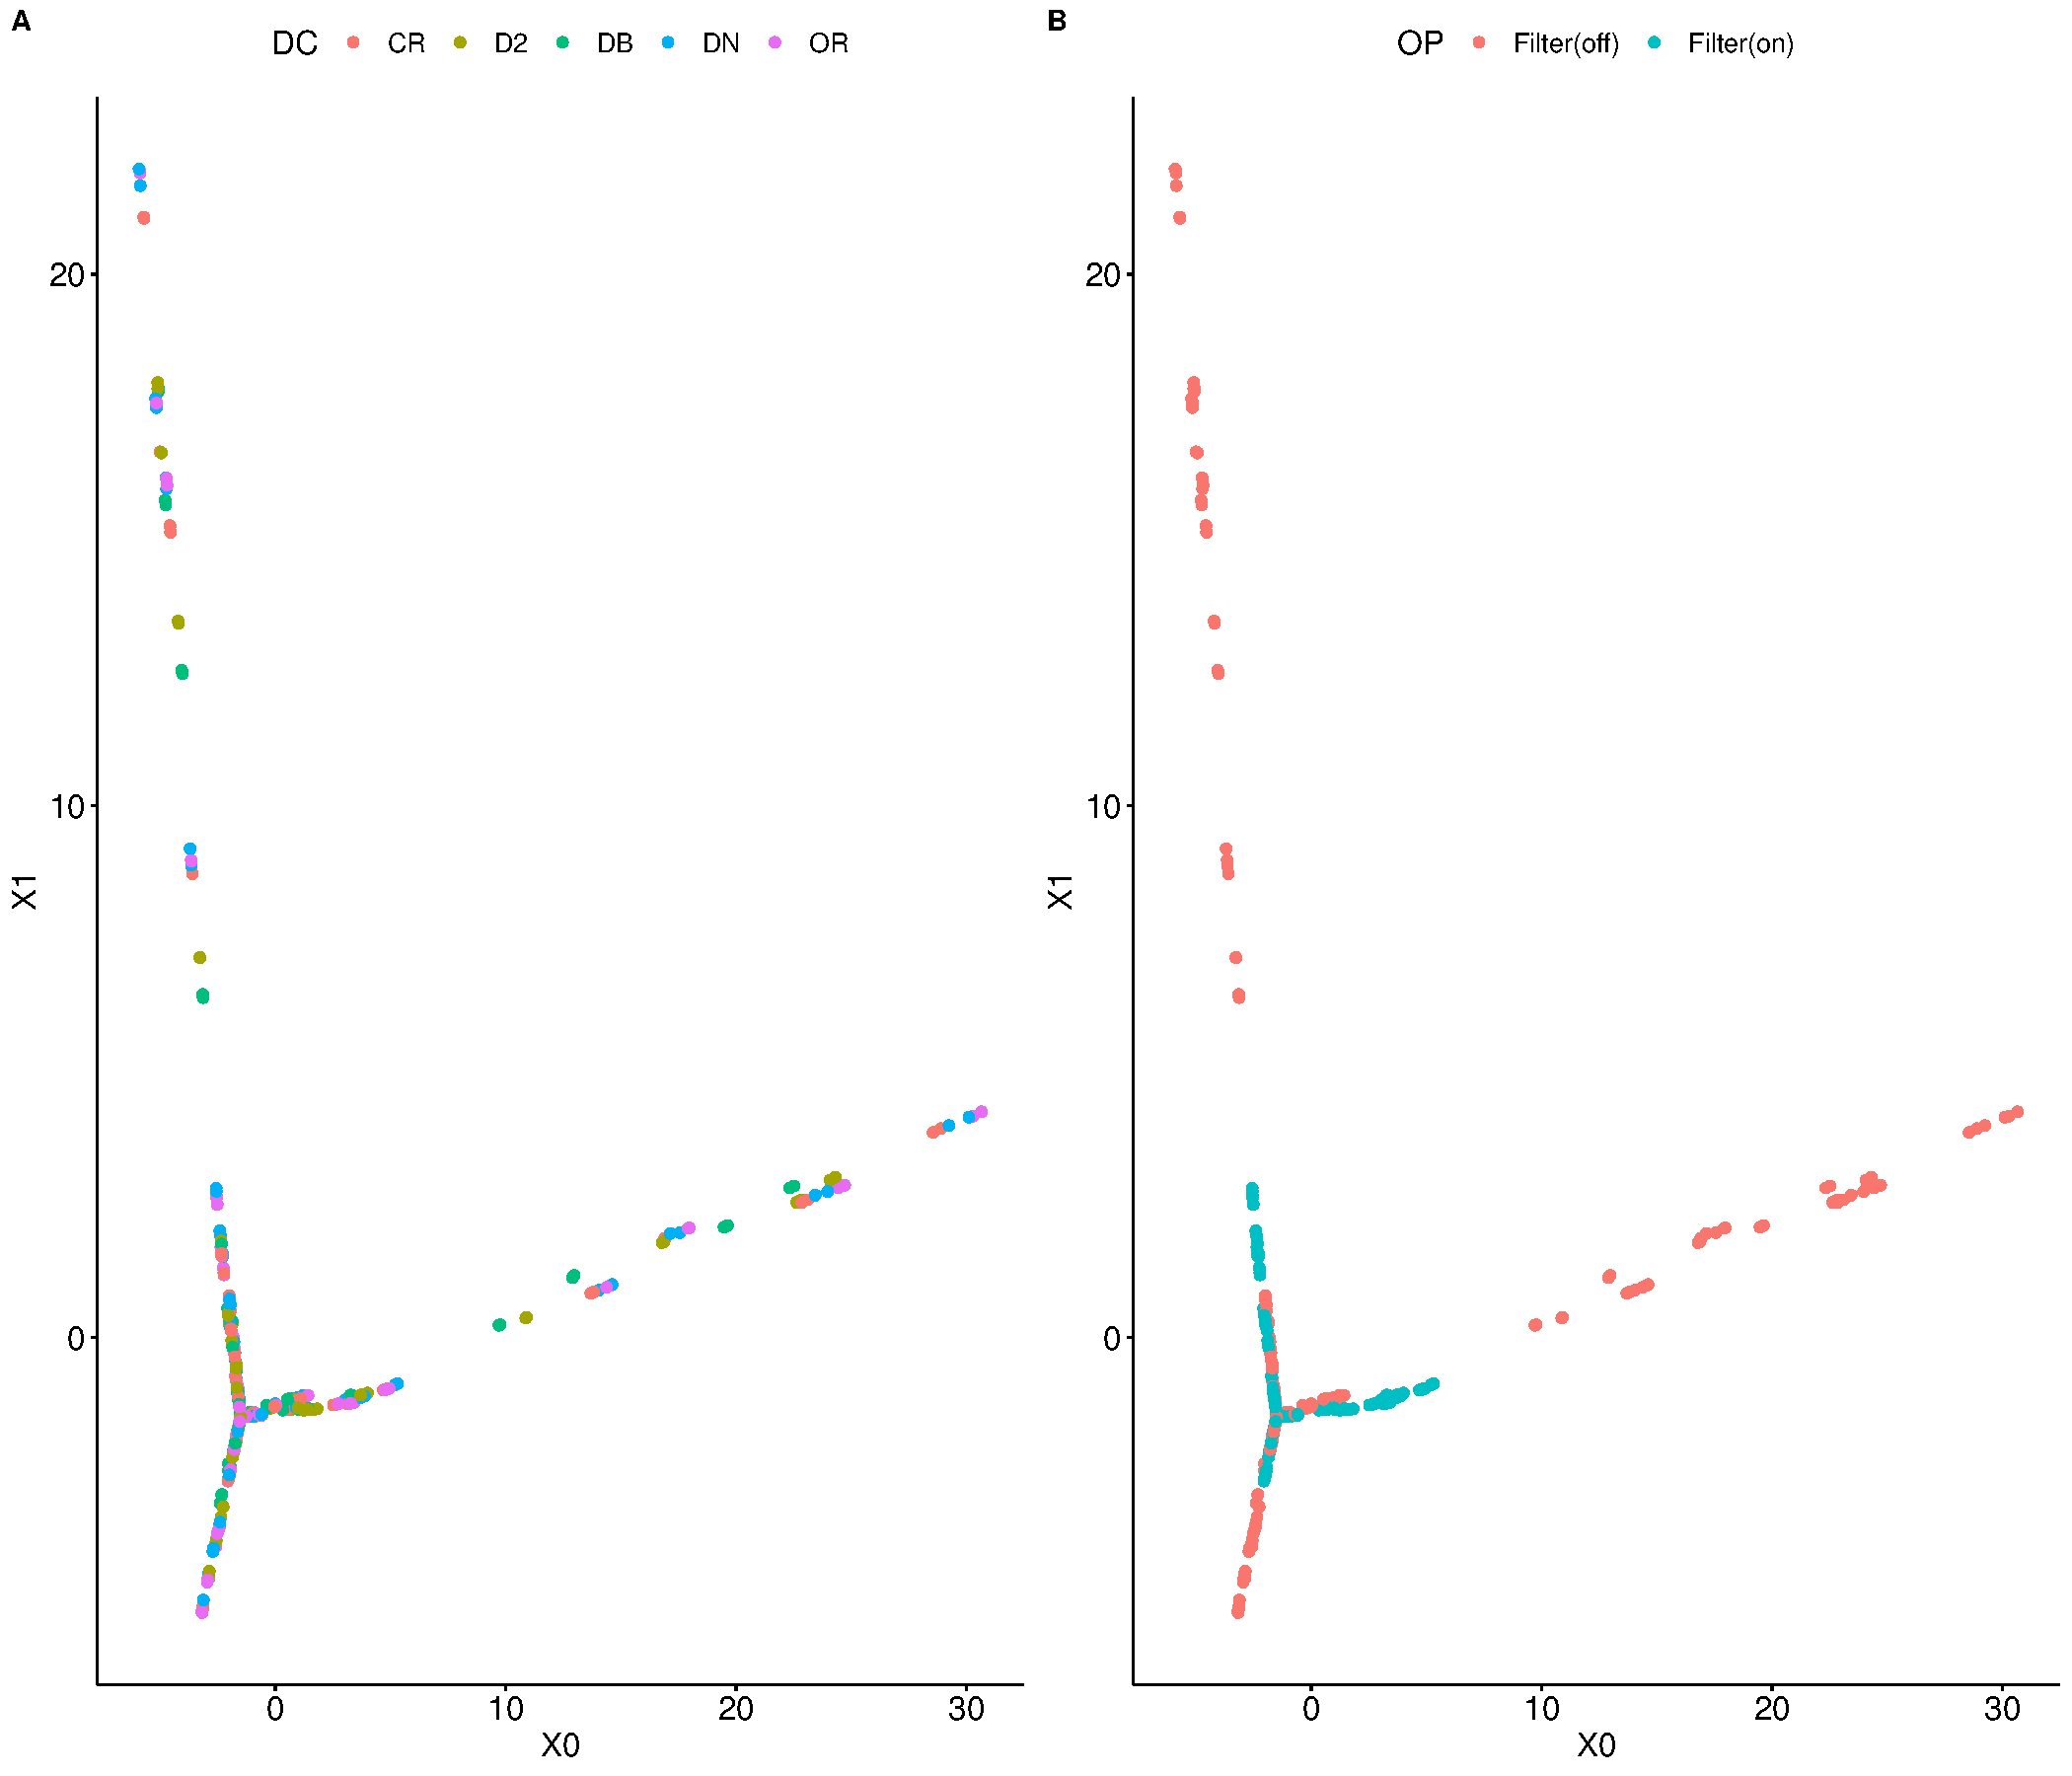
\includegraphics[width=1.0\linewidth]{figure_s1.pdf}
    \end{figure}
    \begin{figure}[H]
      \centering
        \caption{
          \textbf{The variation in the inferred networks in the first two principal axes}
          The plots are colored by the tools or parameters used in the \ac{dc} step (A) and the \ac{op} step (B)
        }
      \label{fig:figure_s1}
    \end{figure}
    \FloatBarrier
    \newpage

    % TODO: Write something about TSNE
    \begin{figure}[H]
      \centering
      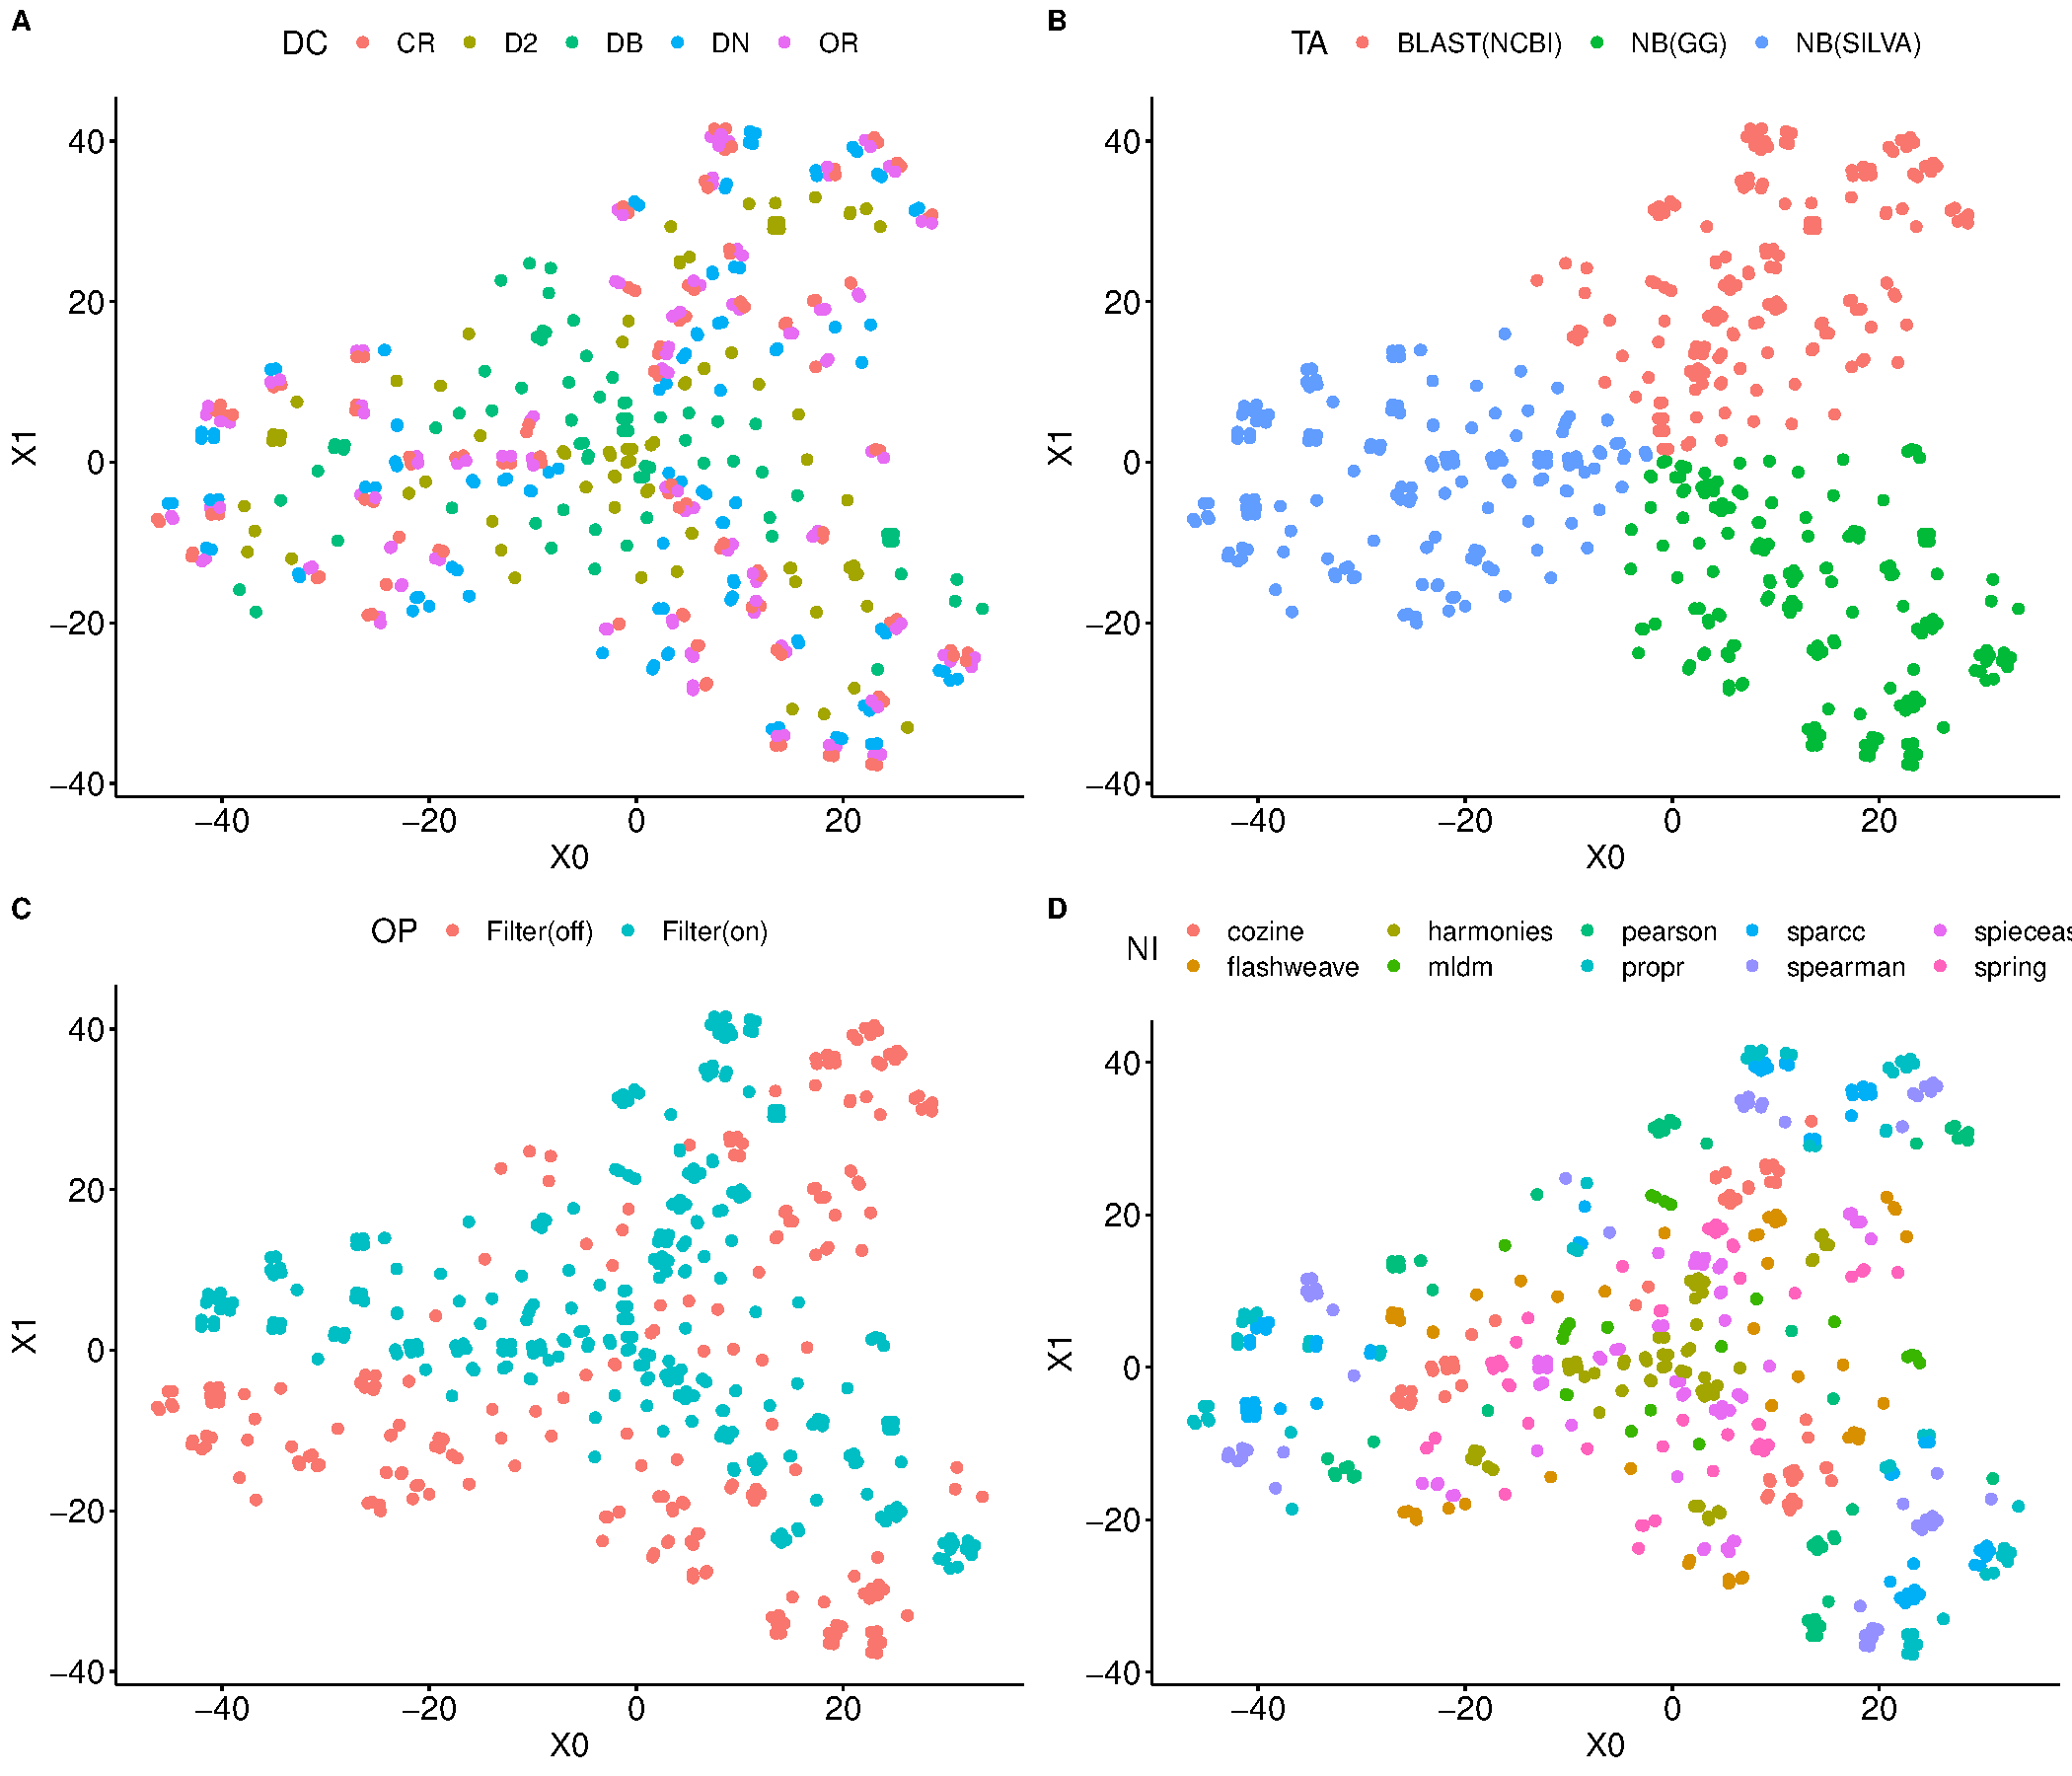
\includegraphics[width=1.0\linewidth]{figure_s2.pdf}
    \end{figure}
    \begin{figure}[H]
      \centering
        \caption{
          \textbf{The TSNE plot of the networks inferred by various methods}.
        }
      \label{fig:figure_s2}
    \end{figure}
    \FloatBarrier
    \newpage


  \subsection*{Similarity of high abundance reference sequences}

    Figure~\ref{fig:figureS3} is similar to Figure~\ref{fig:figure3} shows the average UniFrac distance between reference sequences generated by the various methods in the \ac{dc} step.
    In Figure~\ref{fig:figureS3} however, we use only the top 1000 representative sequences (by abundance) for this calculation.
    We observe that both the weighted and unweighted UniFrac distances are increased compared to the figure with the all the representative sequences.
    This shows that the most abundant representative sequences generated by the methods are not similar to each other.

    \begin{figure}[H]
      \centering
      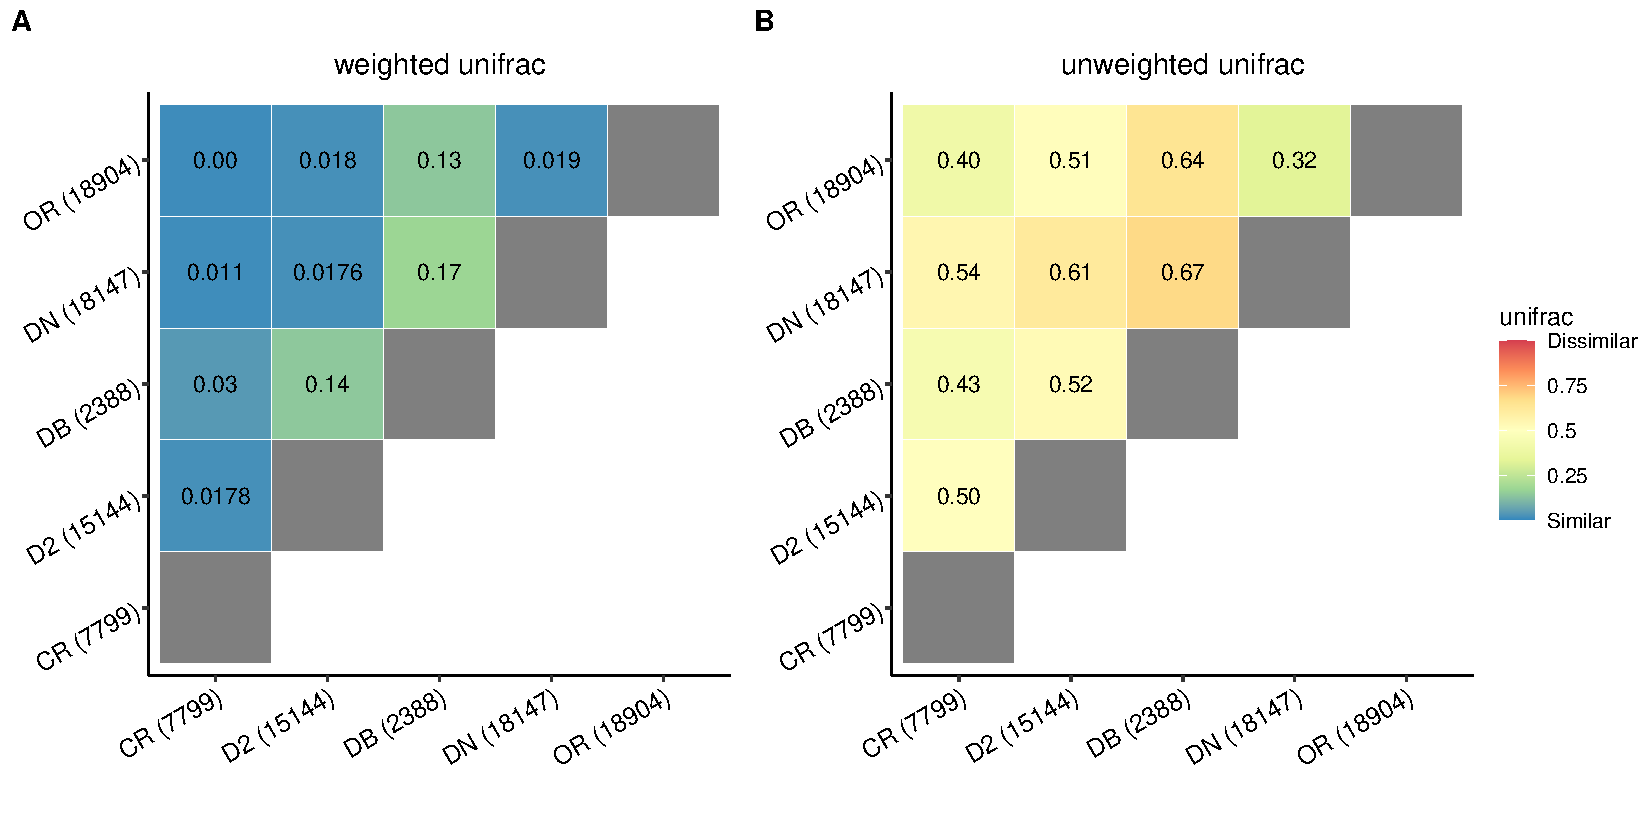
\includegraphics[width=1.0\linewidth]{figure_s3.pdf}
    \end{figure}
    \begin{figure}[H]
      \centering
        \caption{
          \textbf{The UniFrac distance between the 100 most abundant representative sequences generated by various method in the \ac{dc} step}
        }
      \label{fig:figure_s3}
    \end{figure}
    \FloatBarrier
    \newpage

    % TODO: Figure S4 - Unifrac bar plot for CC methods
    \begin{figure}[H]
      \centering
      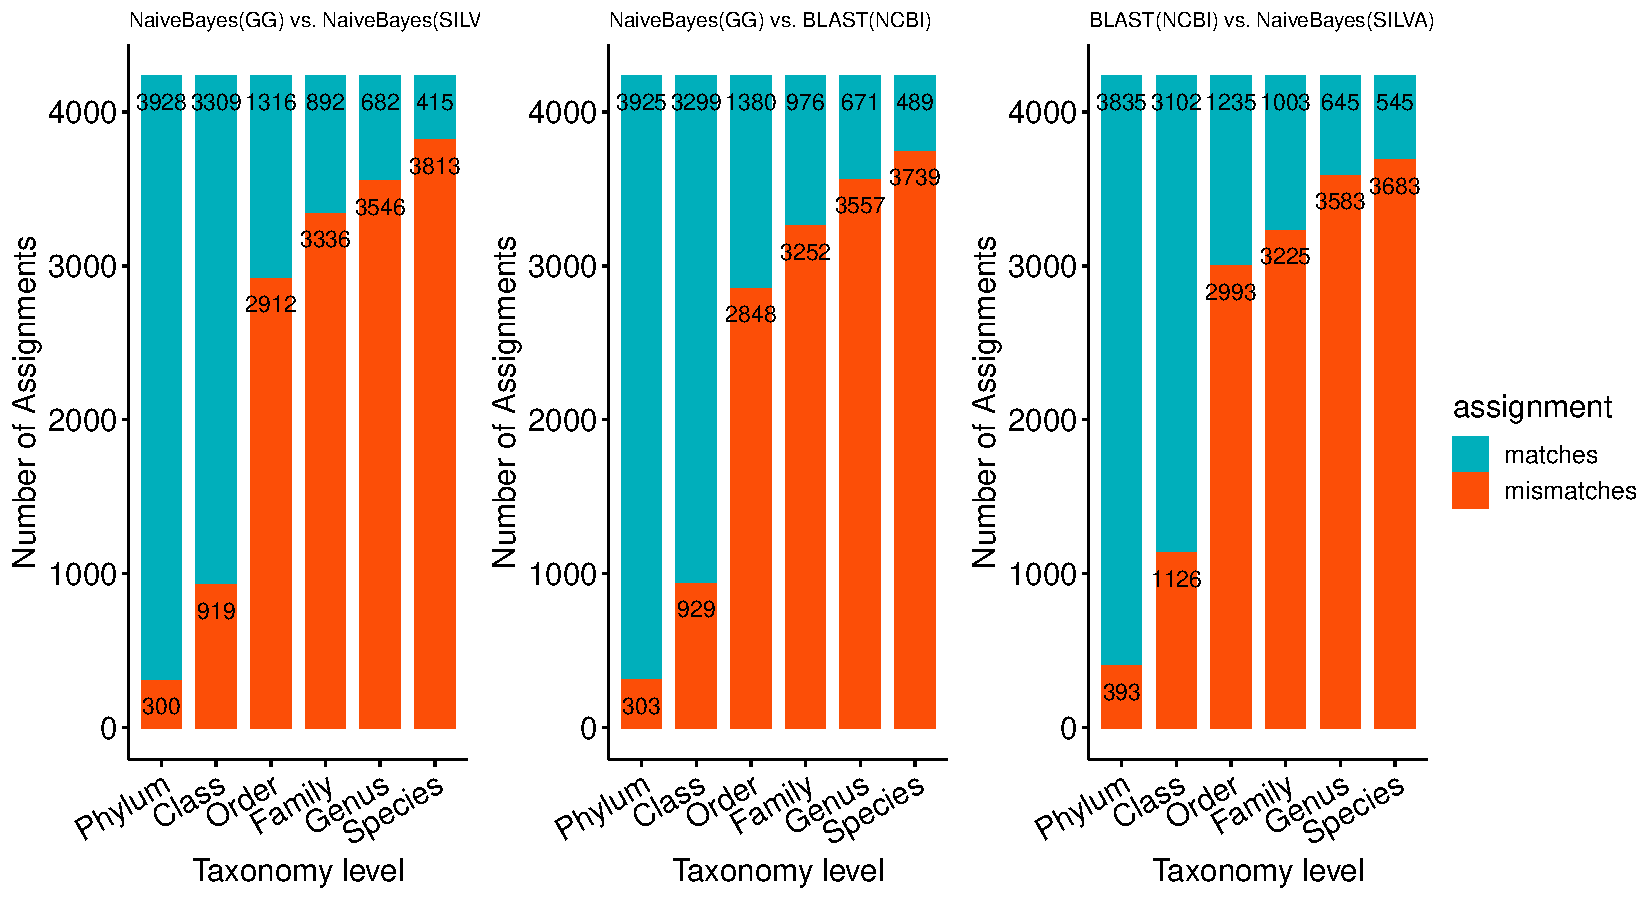
\includegraphics[width=1.0\linewidth]{figure_s4.pdf}
    \end{figure}
    \begin{figure}[H]
      \centering
        \caption{
        }
      \label{fig:figure_s4}
    \end{figure}
    \FloatBarrier
    \newpage

  \subsection*{Mismatches in all assignments at the \ac{TA} step}

    % TODO: Elaborate on this and work on the caption
    Figure~\ref{fig:figure_s5} is similar to Figure~\ref{fig:figure4}B, but instead of the matching only the top 100 taxonomic entities (by abundance), we match all the assignments from one database with those from the other two databases.
    We observe that the percentage of mismatches are indeed higher when considering all the assignments, implying that matching of the taxonomies in the more abundant sequences are more consistent.

    \begin{figure}[H]
      \centering
      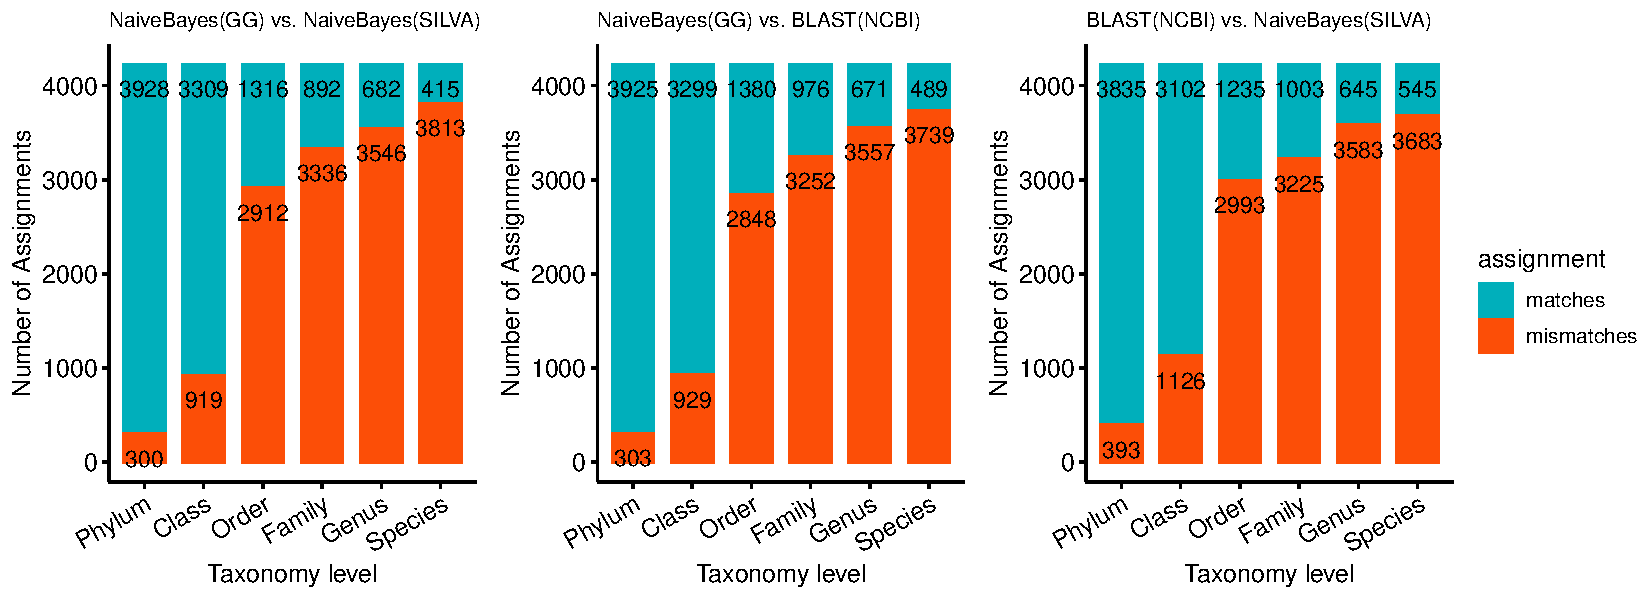
\includegraphics[width=1.0\linewidth]{figure_s5.pdf}
    \end{figure}
    \begin{figure}[H]
      \centering
        \caption{
        }
      \label{fig:figure_s5}
    \end{figure}
    \FloatBarrier
    \newpage


  \subsection*{Consensus and p-value}

  % FIXME: Update according to the new notation in methods section
  \subsubsection*{p-value merging}
  Fisher~\cite{fisher_224a_1948} proposed that for $k$ independent p-values, each generated by $k$ different methods and denoted by $P_i$, the statistic $\Psi$:
  \begin{equation*}
    \begin{aligned}
        \Psi &= \sum_{i=1}^k -2 \log \left( P_i \right) \\
        \Psi &\sim \chi^2_{2k}
    \end{aligned}
  \end{equation*}

  Brown~\cite{brown_400_1975} extended Fisher's method to dependent p-values by using a re-scaled $\chi^2$ distribution:
  \begin{equation*}
    \Psi \sim c \chi^2_{2f}
  \end{equation*}
  where, $f$ is the degrees of freedom and $c$ is the scale factor and are given by:
  \begin{equation*}
    f = \frac{\mathrm{E}[\Psi]^2}{\mathrm{Var}[\Psi]} ~~~\text{and}~~~ c = \frac{\mathrm{Var}[\Psi]}{2\mathrm{E}[\Psi]} = \frac{k}{f}
  \end{equation*}

  Furthermore, Brown showed that $\mathrm{E}[\Psi]$ and $\mathrm{Var}[\Psi]$ can be calculated directly via a numerical integration:
  \begin{equation*}
    \mathrm{E}[\Psi] = 2k ~~~\text{and}~~~ \mathrm{Var}[\Psi] = 4k + 2\sum_{i<j} \mathrm{Cov}\left( -2\log(P_i), -2\log(P_j) \right)
  \end{equation*}

  Kost and McDermott~\cite{kost_combining_2002} further fit a third-order polynomial to approximate the covariance
  \begin{equation}
    \mathrm{Cov}\left( -2\log(P_i), -2\log(P_j) \right) \approx 3.263 \rho_{ij} + 0.710 \rho_{ij}^2 + 0.027 \rho_{ij}^3
    \label{eqn:covariance-pvalues}
  \end{equation}
  where, $\rho_{ij}$ is the correlation between method $i$ and method $j$

  The final combined p-value~\cite{Poole_Gibbs_Shmulevich_Bernard_Knijnenburg_2016} is then given by:
  \begin{equation}
    \begin{aligned}
        & P_{combined} = 1.0 - \Phi_{2f}\left( \psi / c \right) \\
        \text{where},~ &\psi = -2 \sum_{i=1}^k \log(P_i) ~~~\text{and}~~~ \Phi_{2f} = \mathrm{CDF}\left( \chi^2_{2f} \right)
    \end{aligned}
    \label{eqn:pvalue-combined}
  \end{equation}

  The p-value merging method in \ac{micone} (refer Documentation) uses Equation~\ref{eqn:covariance-pvalues} to estimate the covariance of the pvalues and Equation~\ref{eqn:pvalue-combined} to merge the p-values (obtained from bootstrapping) from the different correlation methods.
  % FIXME: Not sure what our stance on this is?
  Note that we do not use Pearson and Spearman methods in the p-value merging step and these algorithms are only used for demonstration and comparison.
  The combined p-values are used to threshold for significance during the consensus network step.

  % TODO: Write all these sections
  \subsection*{Performance of network inference algorithms on seqtime data}
  \subsection*{The JSON network format}

  \begin{figure}[h]
  \centering
  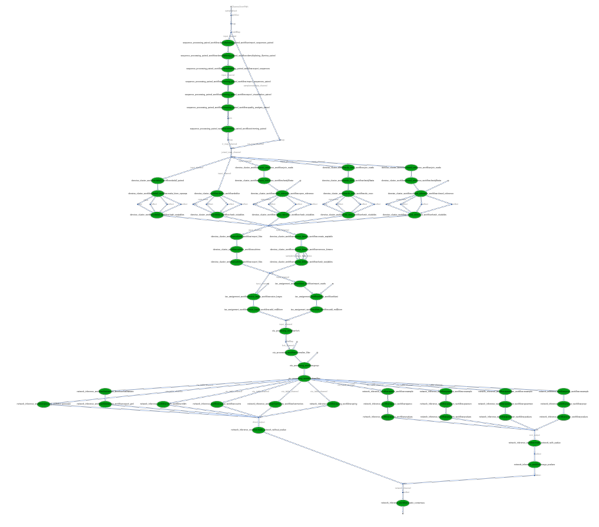
\includegraphics[width=\linewidth]{figureS1.pdf}
  \caption{
    \textbf{Comparison of various denoising and clustering algorithms used in the pipeline}.
    (A, B) Correlation of the abundances of the taxa that are in common between the count matrices created by two different methods.
    (A) The worst correlation (least similar methods) is between open-reference and dada2.
    (B) The best correlation (most similar methods) is between open-reference and denovo.
    (C) A heatmap showing the $\mathrm{R}^2$ of all pairwise comparisons of the methods.
  }
  \label{fig:figureS1}
\end{figure}

  \begin{figure}[h]
    \centering
    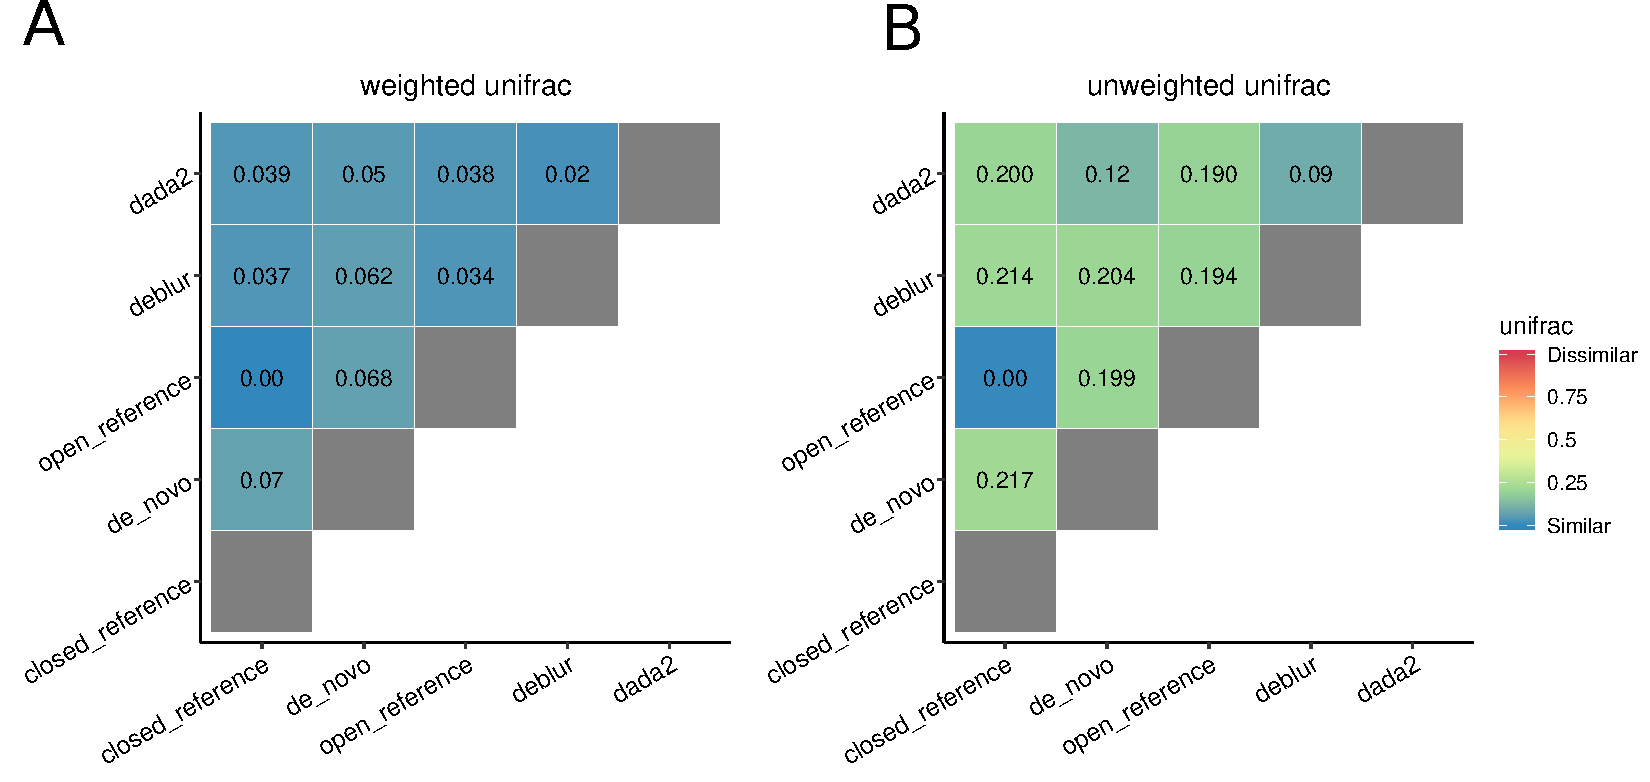
\includegraphics[width=\linewidth]{figureS2.pdf}
    \caption{
      \textbf{Heatmaps showing the weighted and unweighted unifrac distances for the hard palate dataset analysis}.
      (A) weighted unifrac distances and (B) unweighted unifrac distances between the representative sequences generated by different denoising and clustering algorithms.
      These results are in agreement with the stool microbiome dataset.
    }
    \label{fig:figureS2}
  \end{figure}

  \begin{figure}[h]
    \centering
    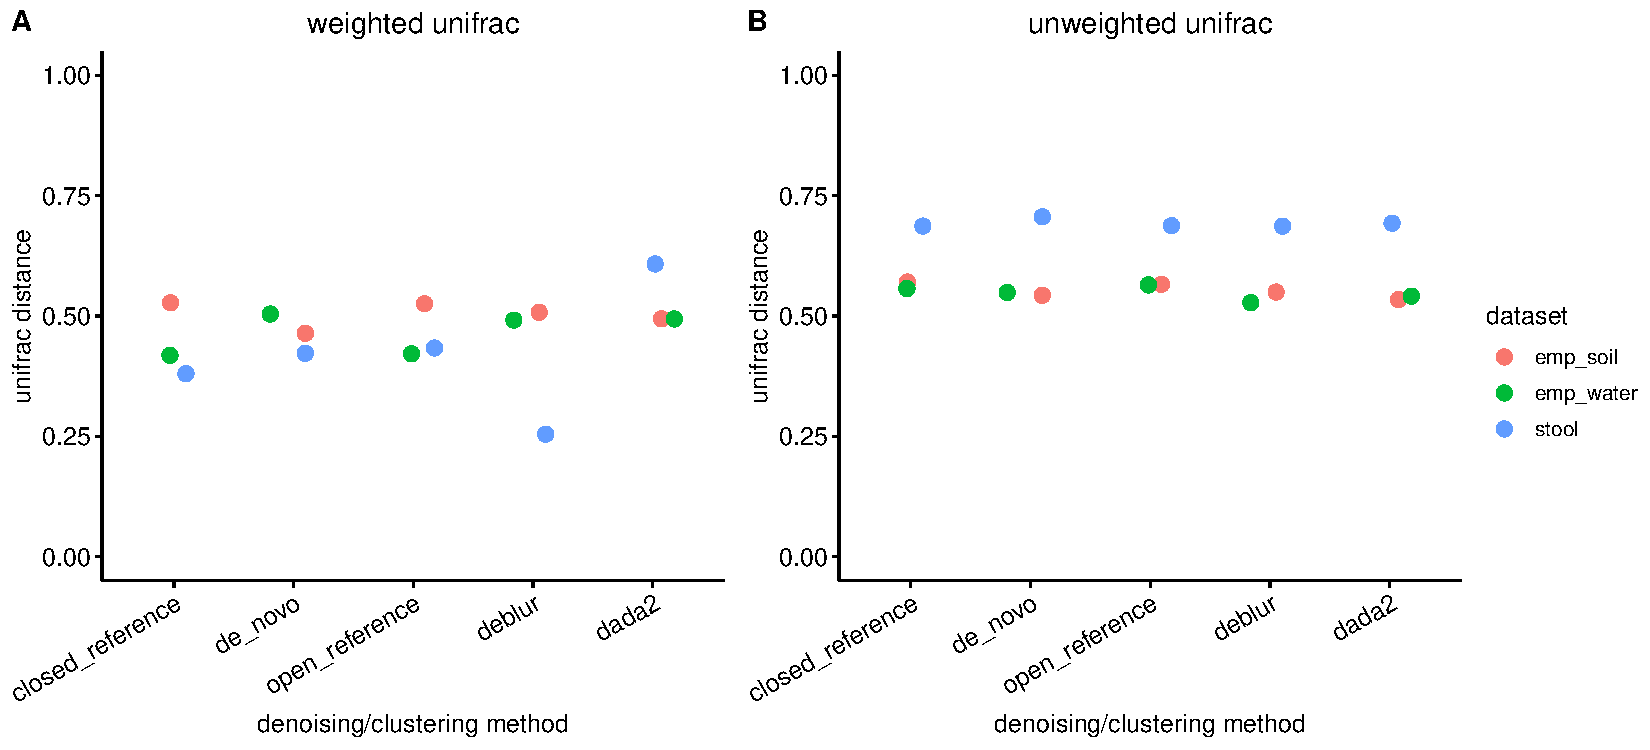
\includegraphics[width=\linewidth]{figureS3.pdf}
    \caption{
      \textbf{The distributions of the average weighted UniFrac distance between the expected sequence profile and the calculated sequence profile in the synthetic datasets}.
      We observe no significant difference between the various methods on the synthetic datasets used for this study.
    }
    \label{fig:figureS3}
  \end{figure}

%   \begin{figure}[h]
%     \centering
%     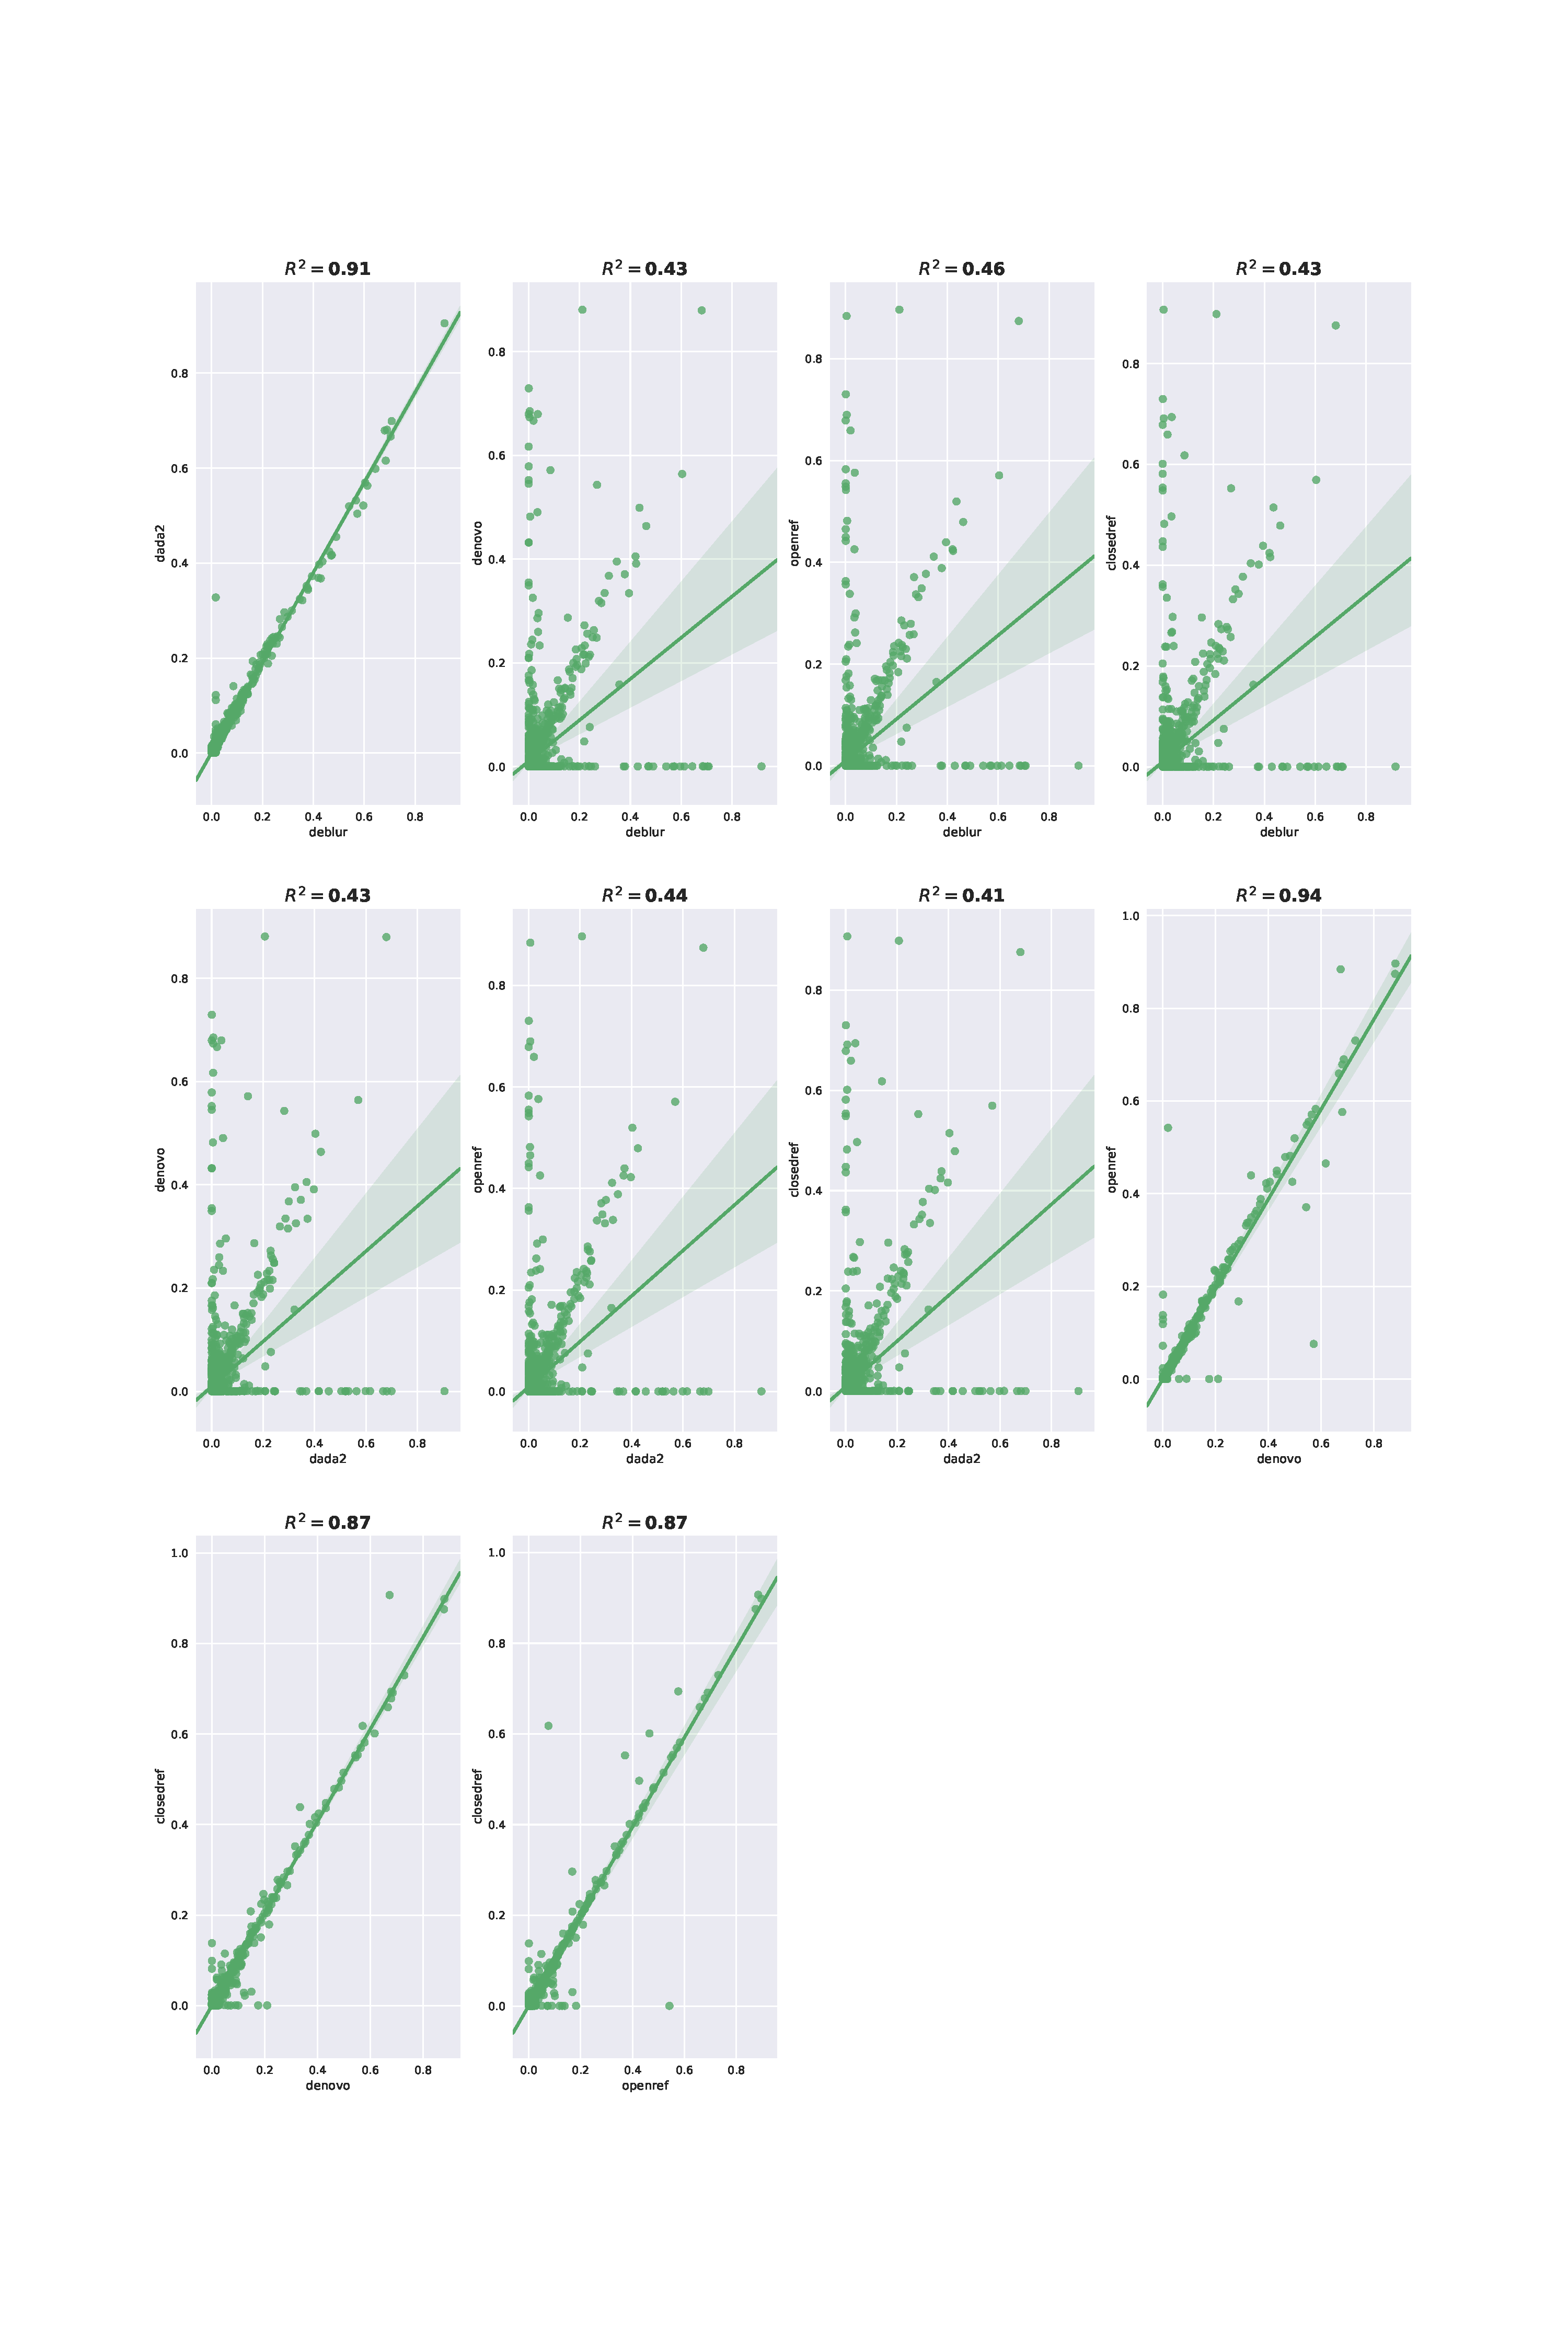
\includegraphics[width=0.9\linewidth]{pdf/all_denoise_reg.pdf}
%     \caption*{All pairwise correlations comparing the similarity between different denoising and clustering methods}
%     \label{fig:figureS4}
%   \end{figure}

  \begin{figure}[h]
    \centering
    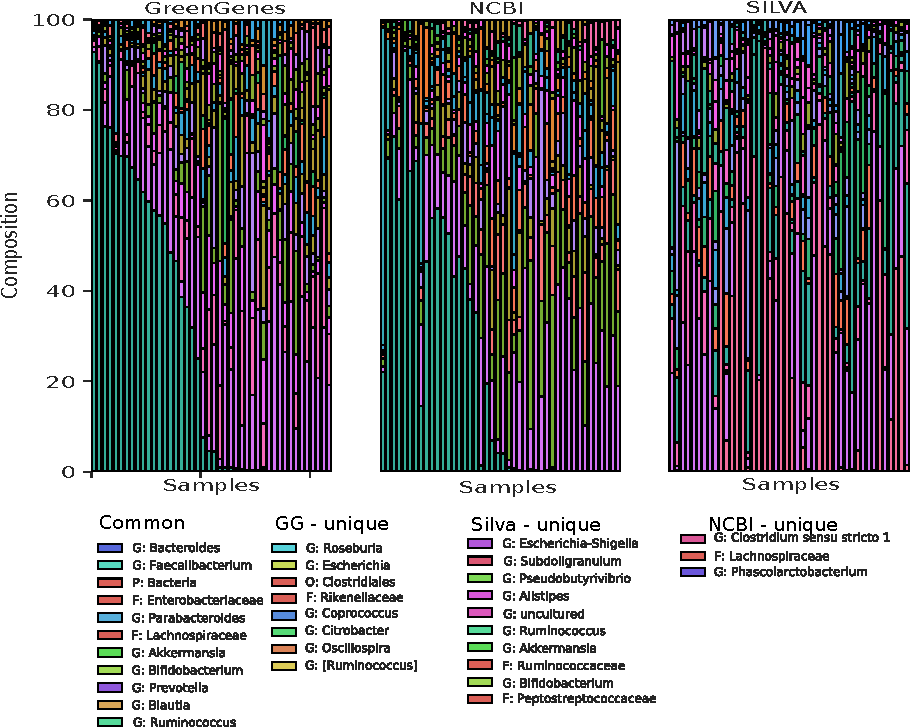
\includegraphics[width=\linewidth]{figureS4.pdf}
    \caption{
      \textbf{(A)} Taxonomy composition of the 20 most abundant genera predicted for the stool microbiome dataset generated using different taxonomy references databases: Greengenes, SILVA and NCBI.
      The legend shows the common and the unique genera among the taxonomy assignments.
  }
    \label{fig:figureS4}
  \end{figure}

  \begin{figure}[h]
    \centering
    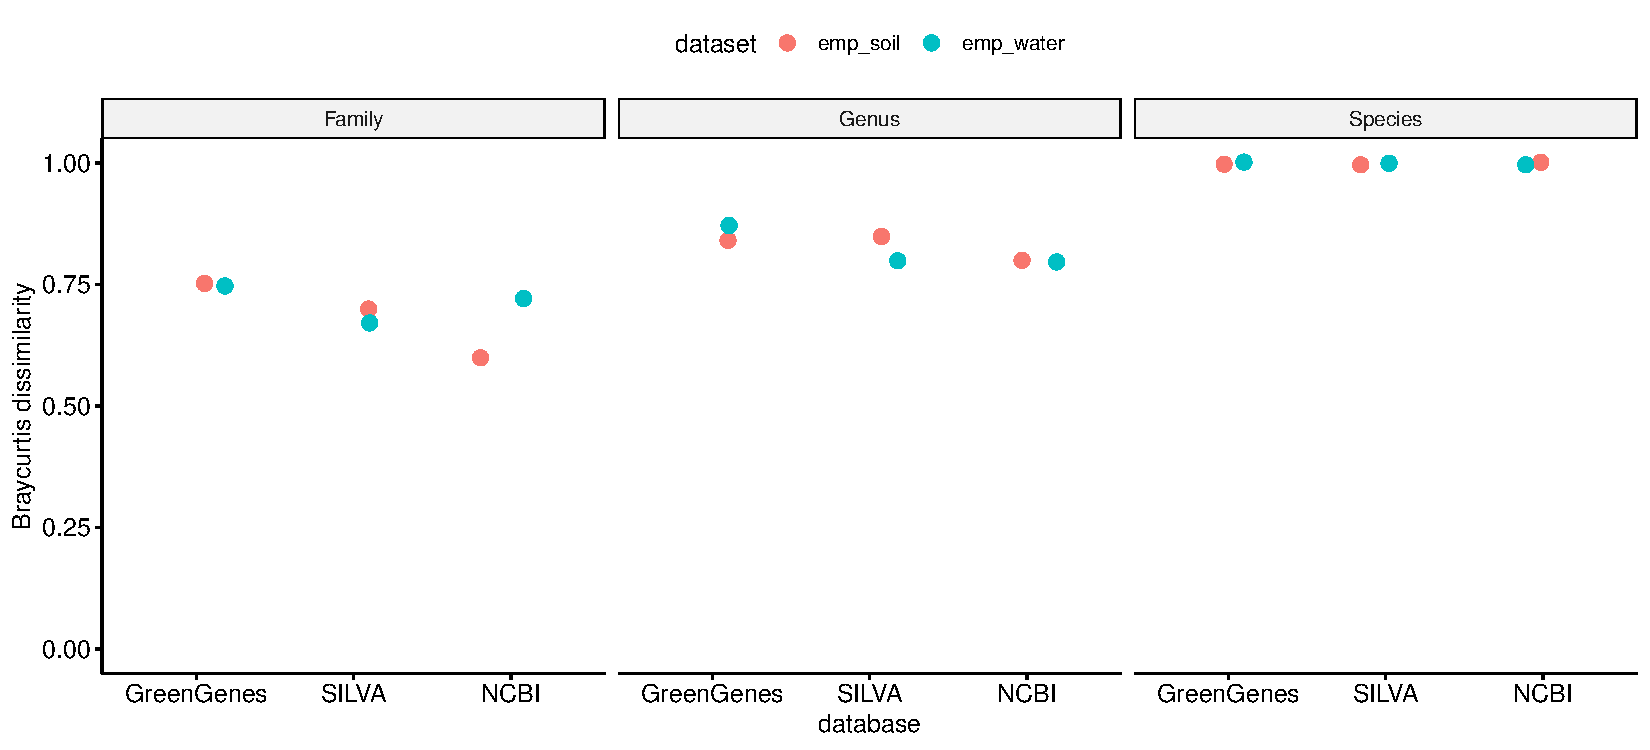
\includegraphics[width=\linewidth]{figureS5.pdf}
    \caption{
      The bray-curtis dissmilarity between the expected taxonomic composition and generated taxonomic composiion for the synthetic datasets.
  }
  \label{fig:figureS5}
  \end{figure}

%   \begin{figure}[h]
%     \centering
%     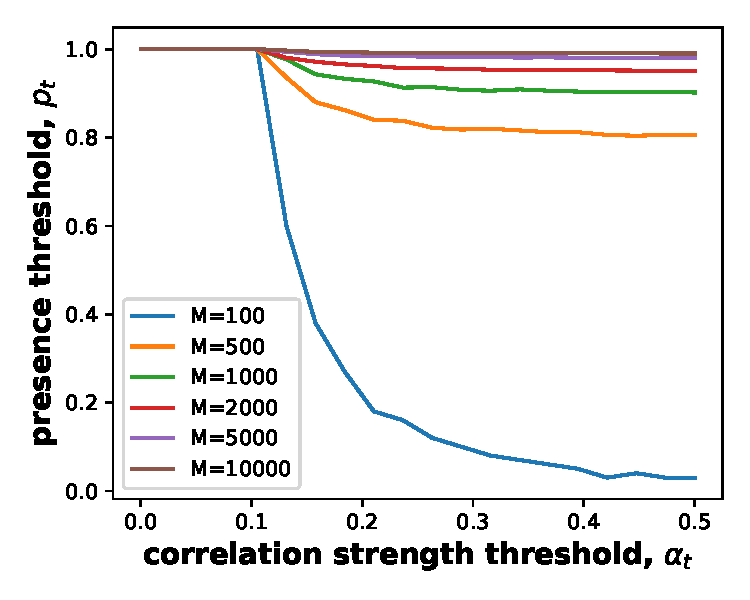
\includegraphics[width=\linewidth]{figureS6.pdf}
%     \caption{
%       Calculation of presence threshold that is applied on the OTU table in the OTU processing (OP) step of the pipeline.
%       This presence threhold $p_t$ is dependent on the number of samples in the dataset and the required correlation stength threshold.
%   }
%     \label{fig:figureS6}
%   \end{figure}

  \begin{figure}[h]
    \centering
    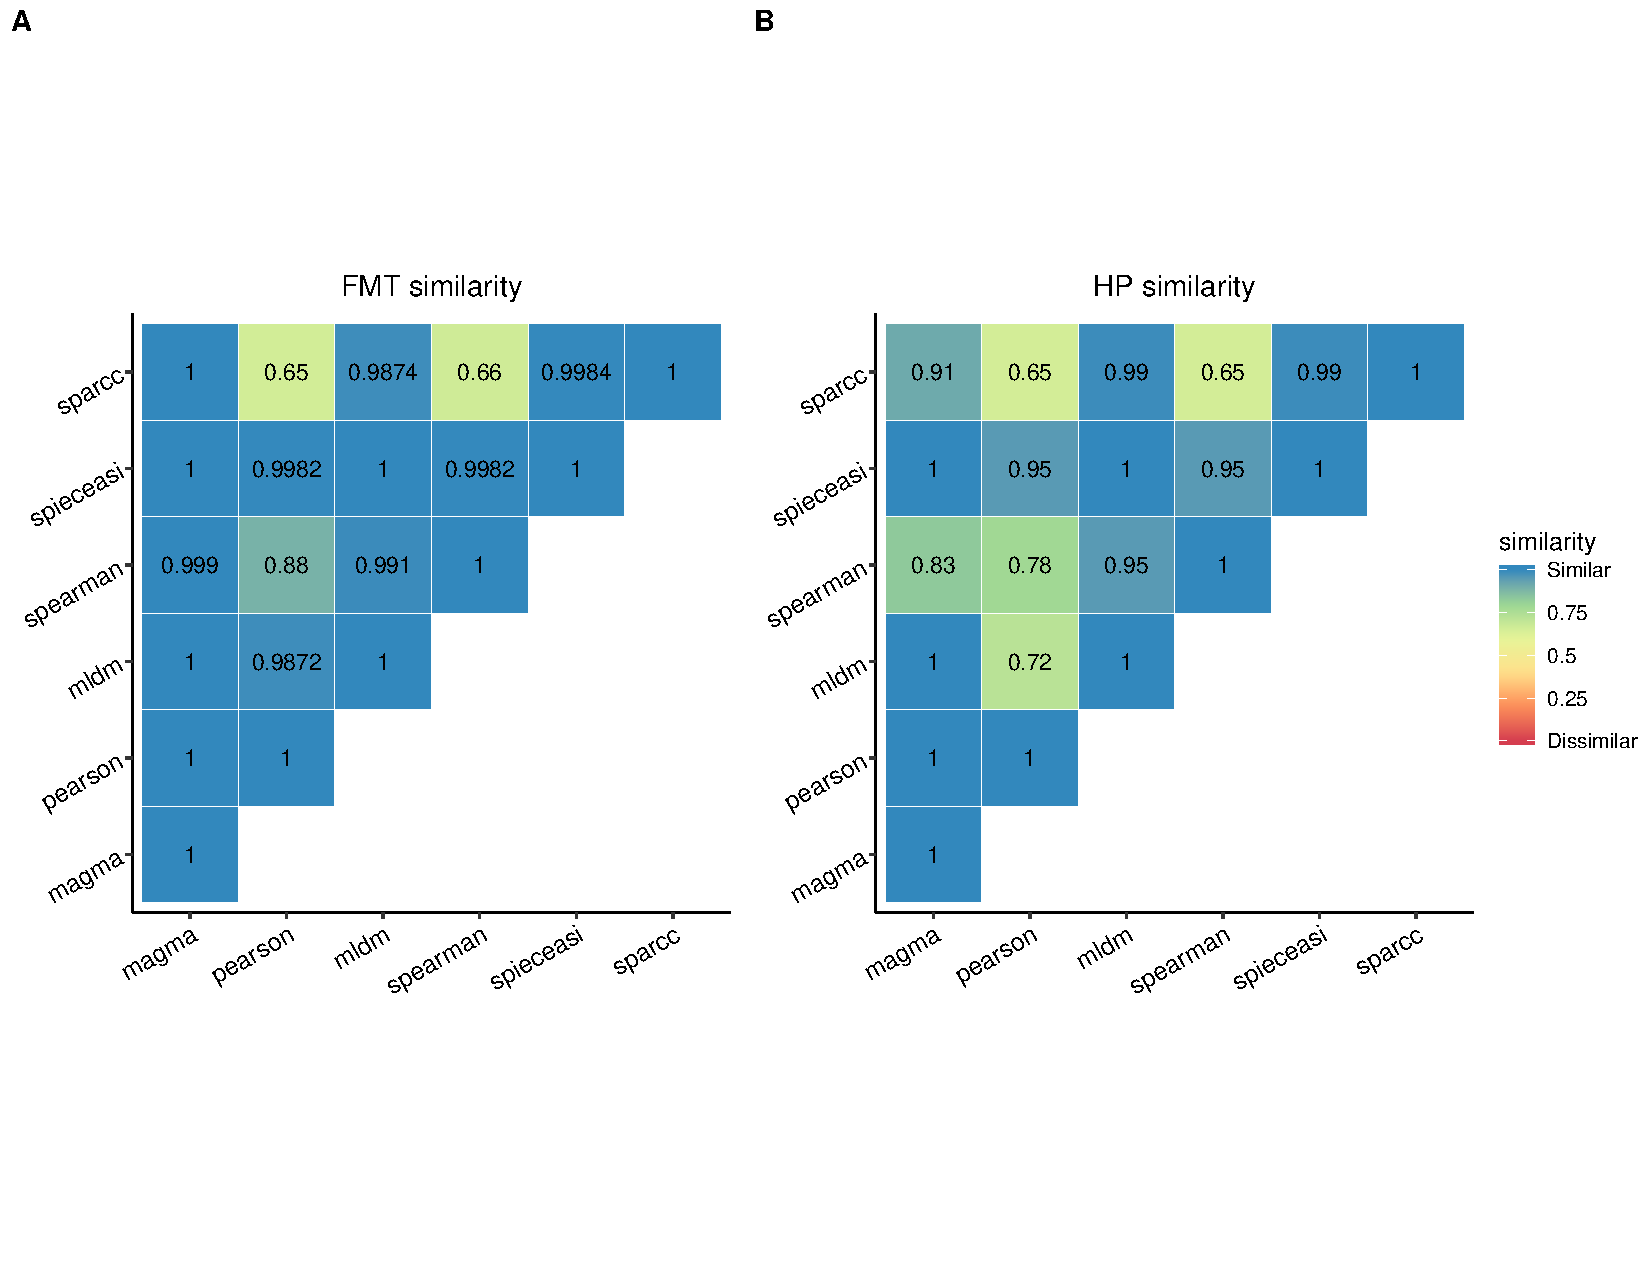
\includegraphics[width=\linewidth]{figureS8.pdf}
    \caption{
      The similarity between the networks generated using the different network inference algorithms for stool dataset (A) and the hard palate dataset (B).
      The similarity between the various methods was found to vary with the dataset used.
  }
    \label{fig:figureS8}
  \end{figure}

  \begin{figure}[h]
    \centering
    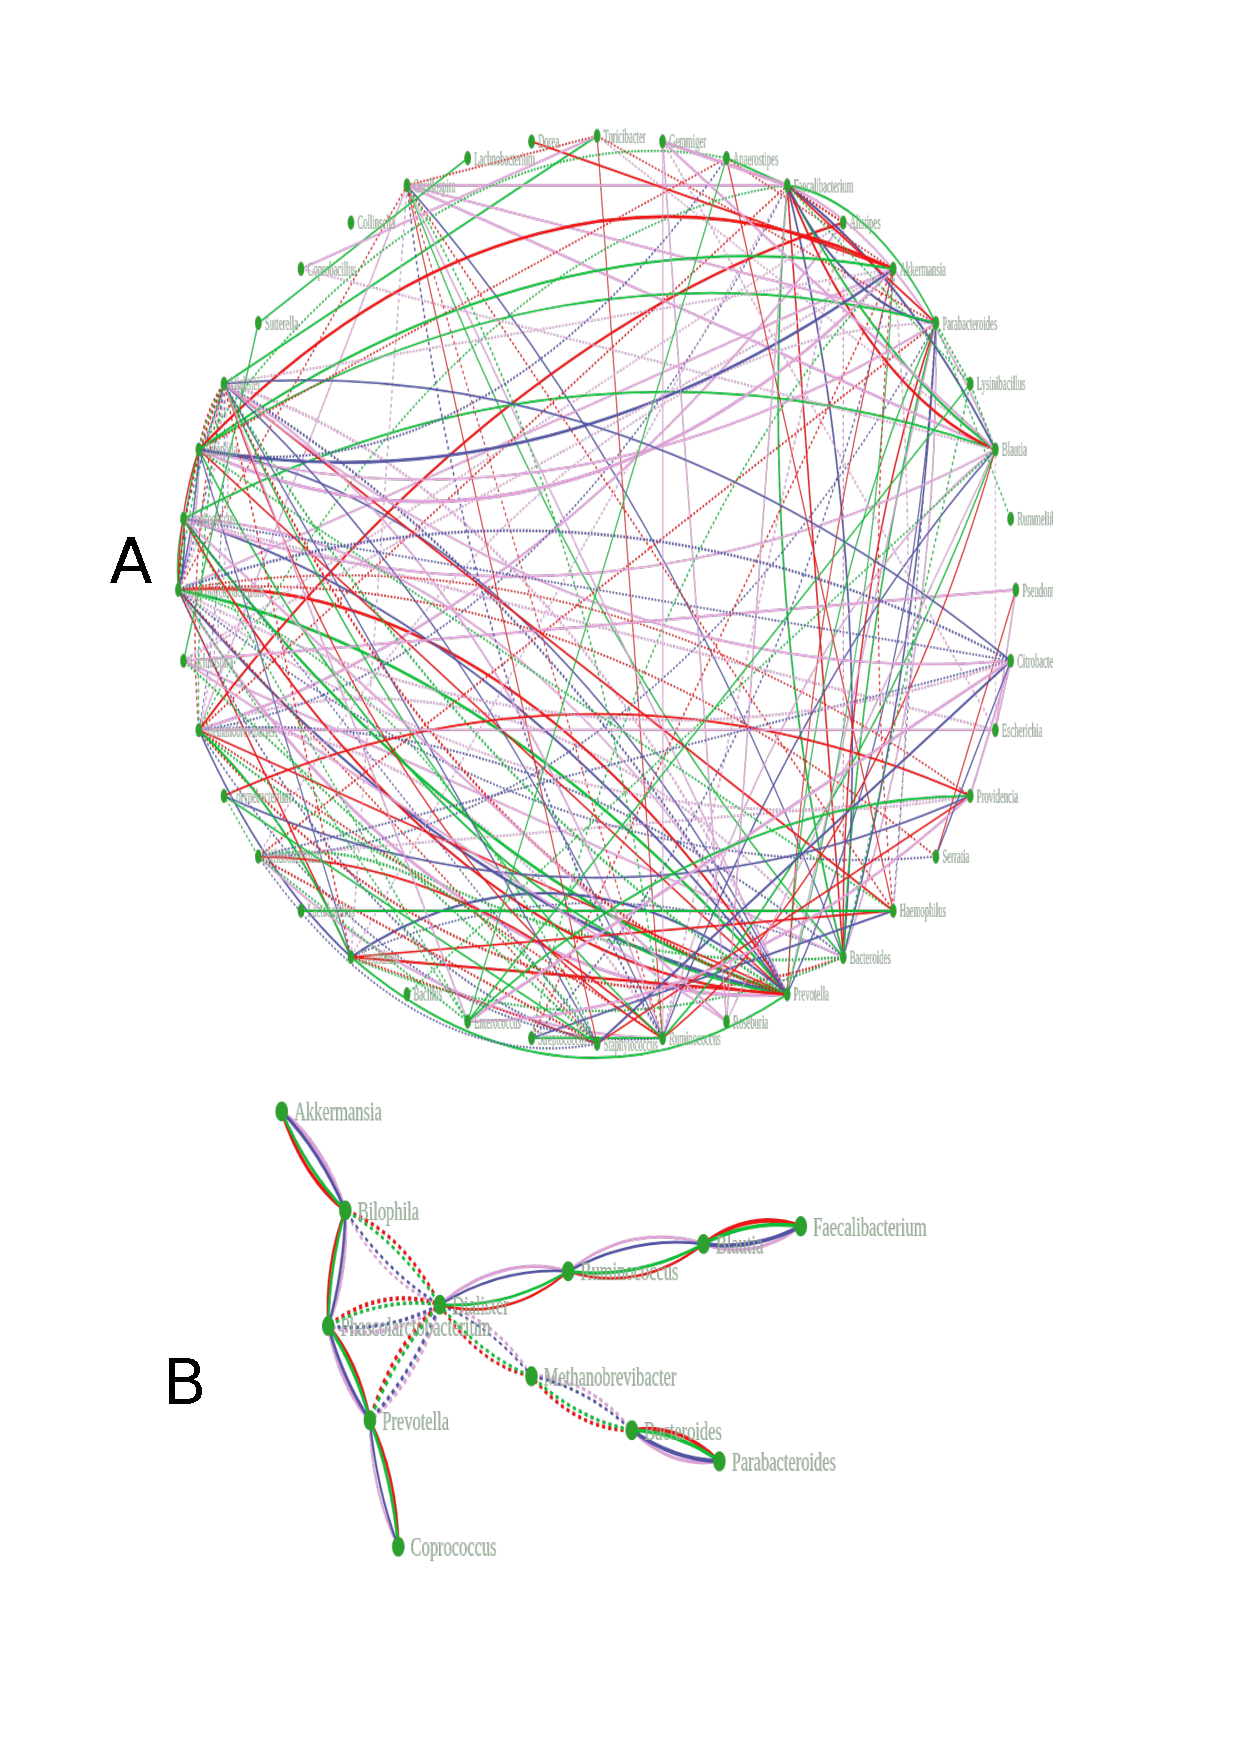
\includegraphics[width=0.8\linewidth]{pdf/denoise_network.pdf}
    \caption{A network showing union (A) and intersection (B) of networks generated using different denoising and clustering tools on the Stool dataset.}
    \label{fig:figureS5}
  \end{figure}


%--------------------------------------------------------%
%   END DOCUMENT
%--------------------------------------------------------%

\end{document}
https://www.overleaf.com/project/5b58887e9f20f9341fd965e6
